% Options for packages loaded elsewhere
\PassOptionsToPackage{unicode}{hyperref}
\PassOptionsToPackage{hyphens}{url}
\PassOptionsToPackage{dvipsnames,svgnames,x11names}{xcolor}
%
\documentclass[
  letterpaper,
  DIV=11,
  numbers=noendperiod]{scrreprt}

\usepackage{amsmath,amssymb}
\usepackage{iftex}
\ifPDFTeX
  \usepackage[T1]{fontenc}
  \usepackage[utf8]{inputenc}
  \usepackage{textcomp} % provide euro and other symbols
\else % if luatex or xetex
  \usepackage{unicode-math}
  \defaultfontfeatures{Scale=MatchLowercase}
  \defaultfontfeatures[\rmfamily]{Ligatures=TeX,Scale=1}
\fi
\usepackage{lmodern}
\ifPDFTeX\else  
    % xetex/luatex font selection
\fi
% Use upquote if available, for straight quotes in verbatim environments
\IfFileExists{upquote.sty}{\usepackage{upquote}}{}
\IfFileExists{microtype.sty}{% use microtype if available
  \usepackage[]{microtype}
  \UseMicrotypeSet[protrusion]{basicmath} % disable protrusion for tt fonts
}{}
\makeatletter
\@ifundefined{KOMAClassName}{% if non-KOMA class
  \IfFileExists{parskip.sty}{%
    \usepackage{parskip}
  }{% else
    \setlength{\parindent}{0pt}
    \setlength{\parskip}{6pt plus 2pt minus 1pt}}
}{% if KOMA class
  \KOMAoptions{parskip=half}}
\makeatother
\usepackage{xcolor}
\setlength{\emergencystretch}{3em} % prevent overfull lines
\setcounter{secnumdepth}{5}
% Make \paragraph and \subparagraph free-standing
\ifx\paragraph\undefined\else
  \let\oldparagraph\paragraph
  \renewcommand{\paragraph}[1]{\oldparagraph{#1}\mbox{}}
\fi
\ifx\subparagraph\undefined\else
  \let\oldsubparagraph\subparagraph
  \renewcommand{\subparagraph}[1]{\oldsubparagraph{#1}\mbox{}}
\fi

\usepackage{color}
\usepackage{fancyvrb}
\newcommand{\VerbBar}{|}
\newcommand{\VERB}{\Verb[commandchars=\\\{\}]}
\DefineVerbatimEnvironment{Highlighting}{Verbatim}{commandchars=\\\{\}}
% Add ',fontsize=\small' for more characters per line
\usepackage{framed}
\definecolor{shadecolor}{RGB}{241,243,245}
\newenvironment{Shaded}{\begin{snugshade}}{\end{snugshade}}
\newcommand{\AlertTok}[1]{\textcolor[rgb]{0.68,0.00,0.00}{#1}}
\newcommand{\AnnotationTok}[1]{\textcolor[rgb]{0.37,0.37,0.37}{#1}}
\newcommand{\AttributeTok}[1]{\textcolor[rgb]{0.40,0.45,0.13}{#1}}
\newcommand{\BaseNTok}[1]{\textcolor[rgb]{0.68,0.00,0.00}{#1}}
\newcommand{\BuiltInTok}[1]{\textcolor[rgb]{0.00,0.23,0.31}{#1}}
\newcommand{\CharTok}[1]{\textcolor[rgb]{0.13,0.47,0.30}{#1}}
\newcommand{\CommentTok}[1]{\textcolor[rgb]{0.37,0.37,0.37}{#1}}
\newcommand{\CommentVarTok}[1]{\textcolor[rgb]{0.37,0.37,0.37}{\textit{#1}}}
\newcommand{\ConstantTok}[1]{\textcolor[rgb]{0.56,0.35,0.01}{#1}}
\newcommand{\ControlFlowTok}[1]{\textcolor[rgb]{0.00,0.23,0.31}{#1}}
\newcommand{\DataTypeTok}[1]{\textcolor[rgb]{0.68,0.00,0.00}{#1}}
\newcommand{\DecValTok}[1]{\textcolor[rgb]{0.68,0.00,0.00}{#1}}
\newcommand{\DocumentationTok}[1]{\textcolor[rgb]{0.37,0.37,0.37}{\textit{#1}}}
\newcommand{\ErrorTok}[1]{\textcolor[rgb]{0.68,0.00,0.00}{#1}}
\newcommand{\ExtensionTok}[1]{\textcolor[rgb]{0.00,0.23,0.31}{#1}}
\newcommand{\FloatTok}[1]{\textcolor[rgb]{0.68,0.00,0.00}{#1}}
\newcommand{\FunctionTok}[1]{\textcolor[rgb]{0.28,0.35,0.67}{#1}}
\newcommand{\ImportTok}[1]{\textcolor[rgb]{0.00,0.46,0.62}{#1}}
\newcommand{\InformationTok}[1]{\textcolor[rgb]{0.37,0.37,0.37}{#1}}
\newcommand{\KeywordTok}[1]{\textcolor[rgb]{0.00,0.23,0.31}{#1}}
\newcommand{\NormalTok}[1]{\textcolor[rgb]{0.00,0.23,0.31}{#1}}
\newcommand{\OperatorTok}[1]{\textcolor[rgb]{0.37,0.37,0.37}{#1}}
\newcommand{\OtherTok}[1]{\textcolor[rgb]{0.00,0.23,0.31}{#1}}
\newcommand{\PreprocessorTok}[1]{\textcolor[rgb]{0.68,0.00,0.00}{#1}}
\newcommand{\RegionMarkerTok}[1]{\textcolor[rgb]{0.00,0.23,0.31}{#1}}
\newcommand{\SpecialCharTok}[1]{\textcolor[rgb]{0.37,0.37,0.37}{#1}}
\newcommand{\SpecialStringTok}[1]{\textcolor[rgb]{0.13,0.47,0.30}{#1}}
\newcommand{\StringTok}[1]{\textcolor[rgb]{0.13,0.47,0.30}{#1}}
\newcommand{\VariableTok}[1]{\textcolor[rgb]{0.07,0.07,0.07}{#1}}
\newcommand{\VerbatimStringTok}[1]{\textcolor[rgb]{0.13,0.47,0.30}{#1}}
\newcommand{\WarningTok}[1]{\textcolor[rgb]{0.37,0.37,0.37}{\textit{#1}}}

\providecommand{\tightlist}{%
  \setlength{\itemsep}{0pt}\setlength{\parskip}{0pt}}\usepackage{longtable,booktabs,array}
\usepackage{calc} % for calculating minipage widths
% Correct order of tables after \paragraph or \subparagraph
\usepackage{etoolbox}
\makeatletter
\patchcmd\longtable{\par}{\if@noskipsec\mbox{}\fi\par}{}{}
\makeatother
% Allow footnotes in longtable head/foot
\IfFileExists{footnotehyper.sty}{\usepackage{footnotehyper}}{\usepackage{footnote}}
\makesavenoteenv{longtable}
\usepackage{graphicx}
\makeatletter
\def\maxwidth{\ifdim\Gin@nat@width>\linewidth\linewidth\else\Gin@nat@width\fi}
\def\maxheight{\ifdim\Gin@nat@height>\textheight\textheight\else\Gin@nat@height\fi}
\makeatother
% Scale images if necessary, so that they will not overflow the page
% margins by default, and it is still possible to overwrite the defaults
% using explicit options in \includegraphics[width, height, ...]{}
\setkeys{Gin}{width=\maxwidth,height=\maxheight,keepaspectratio}
% Set default figure placement to htbp
\makeatletter
\def\fps@figure{htbp}
\makeatother
\newlength{\cslhangindent}
\setlength{\cslhangindent}{1.5em}
\newlength{\csllabelwidth}
\setlength{\csllabelwidth}{3em}
\newlength{\cslentryspacingunit} % times entry-spacing
\setlength{\cslentryspacingunit}{\parskip}
\newenvironment{CSLReferences}[2] % #1 hanging-ident, #2 entry spacing
 {% don't indent paragraphs
  \setlength{\parindent}{0pt}
  % turn on hanging indent if param 1 is 1
  \ifodd #1
  \let\oldpar\par
  \def\par{\hangindent=\cslhangindent\oldpar}
  \fi
  % set entry spacing
  \setlength{\parskip}{#2\cslentryspacingunit}
 }%
 {}
\usepackage{calc}
\newcommand{\CSLBlock}[1]{#1\hfill\break}
\newcommand{\CSLLeftMargin}[1]{\parbox[t]{\csllabelwidth}{#1}}
\newcommand{\CSLRightInline}[1]{\parbox[t]{\linewidth - \csllabelwidth}{#1}\break}
\newcommand{\CSLIndent}[1]{\hspace{\cslhangindent}#1}

\KOMAoption{captions}{tableheading}
\makeatletter
\makeatother
\makeatletter
\@ifpackageloaded{bookmark}{}{\usepackage{bookmark}}
\makeatother
\makeatletter
\@ifpackageloaded{caption}{}{\usepackage{caption}}
\AtBeginDocument{%
\ifdefined\contentsname
  \renewcommand*\contentsname{Table of contents}
\else
  \newcommand\contentsname{Table of contents}
\fi
\ifdefined\listfigurename
  \renewcommand*\listfigurename{List of Figures}
\else
  \newcommand\listfigurename{List of Figures}
\fi
\ifdefined\listtablename
  \renewcommand*\listtablename{List of Tables}
\else
  \newcommand\listtablename{List of Tables}
\fi
\ifdefined\figurename
  \renewcommand*\figurename{Figure}
\else
  \newcommand\figurename{Figure}
\fi
\ifdefined\tablename
  \renewcommand*\tablename{Table}
\else
  \newcommand\tablename{Table}
\fi
}
\@ifpackageloaded{float}{}{\usepackage{float}}
\floatstyle{ruled}
\@ifundefined{c@chapter}{\newfloat{codelisting}{h}{lop}}{\newfloat{codelisting}{h}{lop}[chapter]}
\floatname{codelisting}{Listing}
\newcommand*\listoflistings{\listof{codelisting}{List of Listings}}
\makeatother
\makeatletter
\@ifpackageloaded{caption}{}{\usepackage{caption}}
\@ifpackageloaded{subcaption}{}{\usepackage{subcaption}}
\makeatother
\makeatletter
\@ifpackageloaded{tcolorbox}{}{\usepackage[skins,breakable]{tcolorbox}}
\makeatother
\makeatletter
\@ifundefined{shadecolor}{\definecolor{shadecolor}{rgb}{.97, .97, .97}}
\makeatother
\makeatletter
\makeatother
\makeatletter
\makeatother
\ifLuaTeX
  \usepackage{selnolig}  % disable illegal ligatures
\fi
\IfFileExists{bookmark.sty}{\usepackage{bookmark}}{\usepackage{hyperref}}
\IfFileExists{xurl.sty}{\usepackage{xurl}}{} % add URL line breaks if available
\urlstyle{same} % disable monospaced font for URLs
\hypersetup{
  pdftitle={RAM Codebook},
  pdfauthor={Ahmed Mohamoud},
  colorlinks=true,
  linkcolor={blue},
  filecolor={Maroon},
  citecolor={Blue},
  urlcolor={Blue},
  pdfcreator={LaTeX via pandoc}}

\title{RAM Codebook}
\usepackage{etoolbox}
\makeatletter
\providecommand{\subtitle}[1]{% add subtitle to \maketitle
  \apptocmd{\@title}{\par {\large #1 \par}}{}{}
}
\makeatother
\subtitle{Research Assessment \& Monitoring}
\author{Ahmed Mohamoud}
\date{}

\begin{document}
\maketitle
\ifdefined\Shaded\renewenvironment{Shaded}{\begin{tcolorbox}[interior hidden, boxrule=0pt, enhanced, borderline west={3pt}{0pt}{shadecolor}, frame hidden, sharp corners, breakable]}{\end{tcolorbox}}\fi

\renewcommand*\contentsname{Table of contents}
{
\hypersetup{linkcolor=}
\setcounter{tocdepth}{2}
\tableofcontents
}
\bookmarksetup{startatroot}

\hypertarget{about-the-guide}{%
\chapter*{About the Guide}\label{about-the-guide}}
\addcontentsline{toc}{chapter}{About the Guide}

\markboth{About the Guide}{About the Guide}

This guide is a collection of ready-to-use packages and scripts designed
to support varous tasks, including the development and testing of data
collection tools, data cleaning and processing through running high
frequency checks and generation of data quality reports. calculation of
WFP cooperate indicators and data analysis. it also features features
WFP branded visualization and tools to effectively communicate results
through reports and dashboards. The guide is build on top of the VAM
Resource Center

\hypertarget{brief-overview}{%
\section*{Brief Overview}\label{brief-overview}}
\addcontentsline{toc}{section}{Brief Overview}

\markright{Brief Overview}

\texttt{Survey\ Planning} will introduce SurveyDesigner and how to adopt
WFP codebook and prepare XLSForms ready for data collection. also it
will cover checking your data collection tools prior data collection by
filling dumpy data to run preliminary tests. also it will cover
accessing MoDa data through the API in order to automate the process of
accessing data throught R Studio.

\texttt{Data\ Cleaning\ \&\ Processing} will cover data quality checking
components including runing high frequency checks on household level
data and logging issues in standarized appraoch of replacing old values
with new values in order to have clean data. also it will cover running
spatial verification checks and generating data quality reports.

\texttt{Indicator\ Calculation} will introduce how to compute WFP
cooperate indicators without adoping long scripts. WFPIndicators package
will provide comprehensive functions for calculating indicators and
users can only provide the required paramers.

\texttt{Data\ Analysis} will provide data analysis functions for
generating results tables and running statistical refrence for the
computed indicators. also it will show how to speedup the process of
generating results from survey data.

\texttt{Data\ Visualization} will provide WFP branded color plates and
charts for visualizing cooperate indicators and as well keeping branded
visuals.

\texttt{Dashboard\ \&\ Reports} will provide markdown reporting
templates for rending branded reports that can be quickly shared with
auidance. also the package will provide Dashboard templates that can be
easily adopted for making information products quickly.

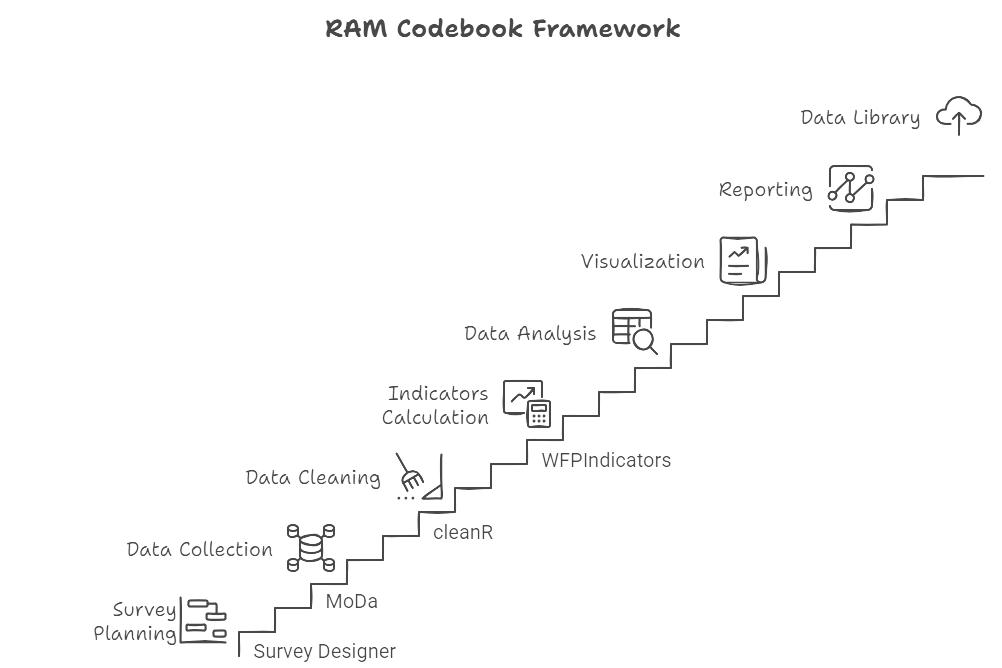
\includegraphics[width=1\textwidth,height=\textheight]{assets/Framework.png}

\hypertarget{about-the-author}{%
\section*{About the Author}\label{about-the-author}}
\addcontentsline{toc}{section}{About the Author}

\markright{About the Author}

\bookmarksetup{startatroot}

\hypertarget{survey-planning}{%
\chapter{Survey Planning}\label{survey-planning}}

\hypertarget{surveydesigner}{%
\section{SurveyDesigner}\label{surveydesigner}}

Survey Designer is an application that allows users in the field to
quickly and easily build standardized assessment and monitoring surveys.
All indicators from the Corporate Results Framework (2022-2025) will be
automatically available for country offices in the Survey Designer, as
well as a variety of other questions and indicators to generate
standardized surveys. Survey Designer allows users to export surveys as
an XLSForm, or directly publish the surveys in MoDa or Kobo.

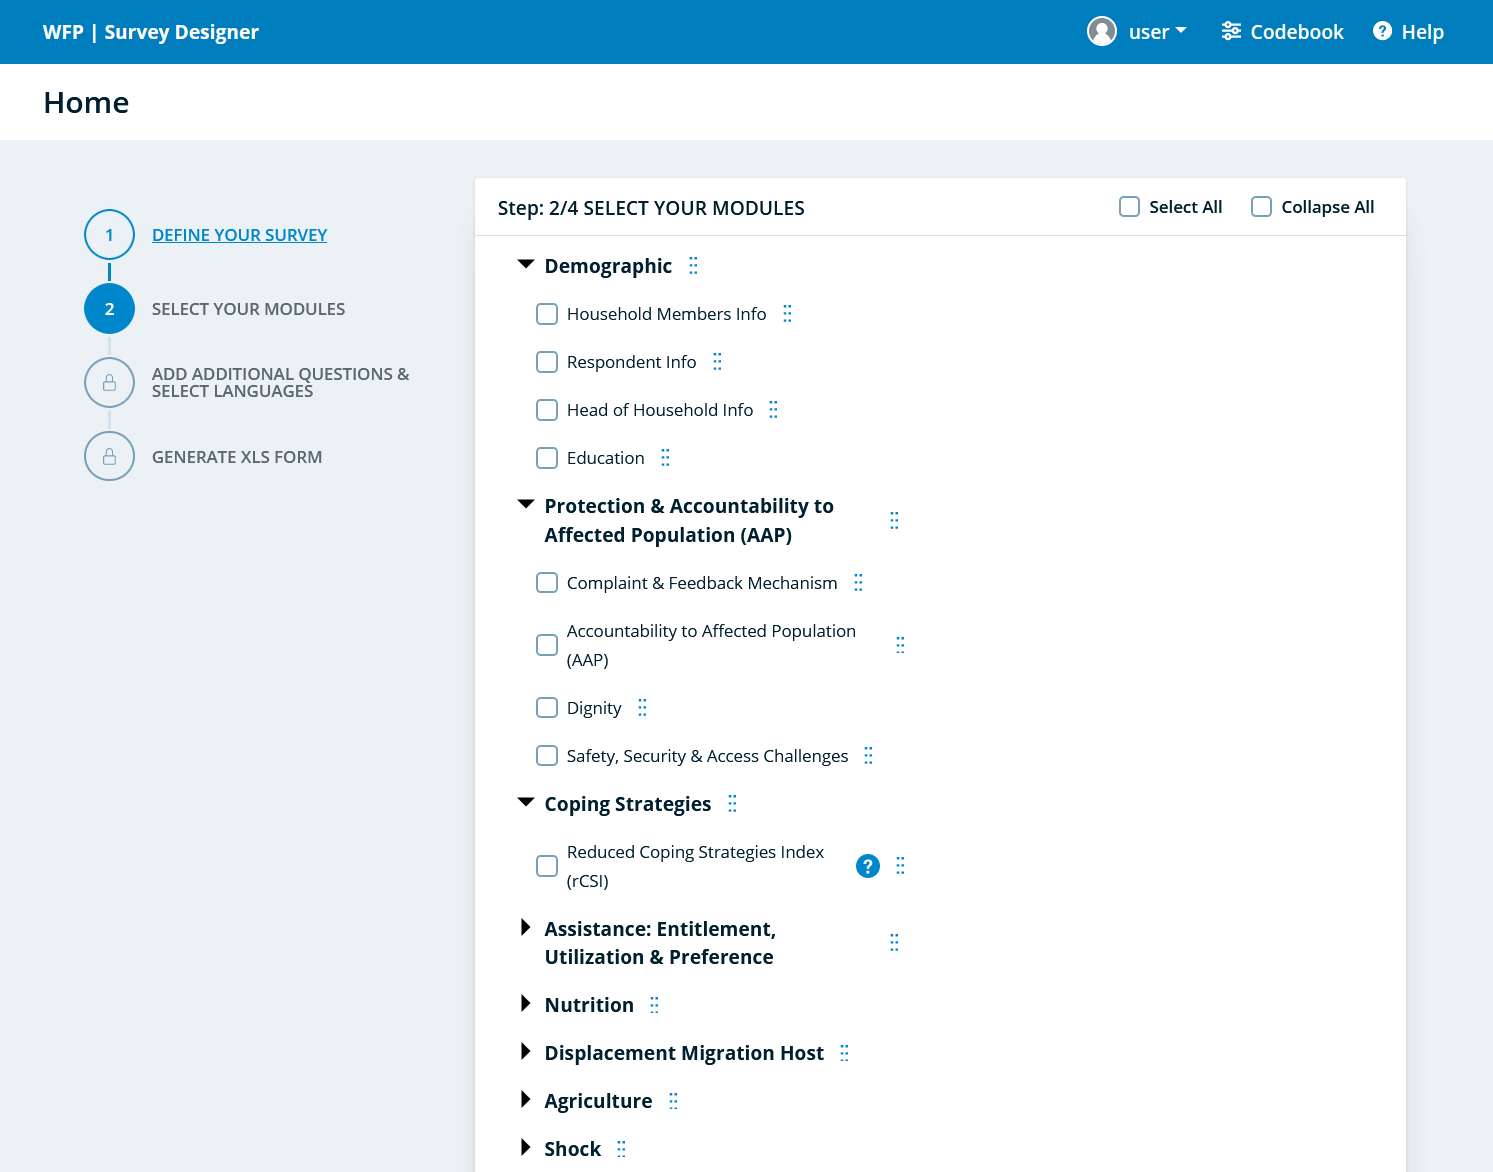
\includegraphics[width=1\textwidth,height=\textheight]{assets/SurveyDesigner.png}

\hypertarget{checking-xslforms}{%
\section{Checking XSLForms}\label{checking-xslforms}}

\hypertarget{downloading-data-from-moda}{%
\section{Downloading Data from MoDa}\label{downloading-data-from-moda}}

You can download data from MoDa server through the API using
modadownloader package. its prety straght forward and you need to
provide your project initial and token information. reproducible example
can be found in the below;

\begin{Shaded}
\begin{Highlighting}[]
\CommentTok{\# intall connectmoda from cran}
\CommentTok{\# install.packages("connectoModa")}

\FunctionTok{library}\NormalTok{(connectoModa)}

\CommentTok{\# Example usage to fetch users from MoDA}
\NormalTok{your\_data }\OtherTok{\textless{}{-}} \FunctionTok{get\_user\_moda}\NormalTok{(}\AttributeTok{form\_id =} \DecValTok{56597}\NormalTok{, }\AttributeTok{Token =} \StringTok{"your\_token\_here"}\NormalTok{)}
\end{Highlighting}
\end{Shaded}

\bookmarksetup{startatroot}

\hypertarget{data-cleaning-processing}{%
\chapter{Data Cleaning \& Processing}\label{data-cleaning-processing}}

in each chapter or part of the book, there will be dedicated package, so
please ensure to install pre-requisted packages before runing the codes.

\begin{Shaded}
\begin{Highlighting}[]
\FunctionTok{library}\NormalTok{(tidyverse)}
\FunctionTok{library}\NormalTok{(readxl)}
\FunctionTok{library}\NormalTok{(cleanR)}

\CommentTok{\# survey\_df \textless{}{-} cleanR::survey\_data}

\NormalTok{survey\_df }\OtherTok{\textless{}{-}} \FunctionTok{read\_excel}\NormalTok{(}\StringTok{"input/MoDa\_Data\_2025{-}03{-}13.xlsx"}\NormalTok{)}
\end{Highlighting}
\end{Shaded}

Data processing and cleaning is critical part as it involves high
frequency checks and spot check for survey data to flag issues that need
to be verified and made changes by keeping reference of alterations made
to the original data. There are predetermined quality checks that can be
applied to any data and as well the data officer can draft unique checks
based on the context. This brings the flexibililty of adopting existing
spot checks and as well adding your own checking paratemers to the
process and generate cleaning log book.

\hypertarget{productivity-coverage}{%
\section{Productivity \& Coverage}\label{productivity-coverage}}

topics to work!! to be deleted :) - assessment tracking sheet report -
assessment productivity - daily valid surveys

\hypertarget{survey-coverage}{%
\subsection{Survey Coverage}\label{survey-coverage}}

\begin{Shaded}
\begin{Highlighting}[]
\NormalTok{survey\_tracking }\OtherTok{\textless{}{-}} \FunctionTok{summarise}\NormalTok{(}\FunctionTok{group\_by}\NormalTok{(survey\_df, ADMIN1Name, ADMIN2Name), }\AttributeTok{count =} \FunctionTok{n}\NormalTok{())}
\NormalTok{check\_survey }\OtherTok{\textless{}{-}} \FunctionTok{unique}\NormalTok{(}\FunctionTok{na.omit}\NormalTok{(survey\_df}\SpecialCharTok{$}\NormalTok{today))}
\ControlFlowTok{for}\NormalTok{(j }\ControlFlowTok{in}\NormalTok{ check\_survey)\{}
\NormalTok{  survey\_tracking[, }\FunctionTok{ncol}\NormalTok{(survey\_tracking) }\SpecialCharTok{+}\DecValTok{1}\NormalTok{] }\OtherTok{\textless{}{-}}\NormalTok{ (survey\_df }\SpecialCharTok{\%\textgreater{}\%} 
                                                    \FunctionTok{group\_by}\NormalTok{(ADMIN1Name, ADMIN2Name) }\SpecialCharTok{\%\textgreater{}\%} 
                                                    \FunctionTok{summarise}\NormalTok{(}\AttributeTok{val=}\FunctionTok{sum}\NormalTok{(}\FunctionTok{na.omit}\NormalTok{(today}\SpecialCharTok{==}\NormalTok{j))) }\SpecialCharTok{\%\textgreater{}\%} 
                                                    \FunctionTok{arrange}\NormalTok{(ADMIN1Name, ADMIN2Name)) }\SpecialCharTok{$}\NormalTok{val}
  \FunctionTok{names}\NormalTok{(survey\_tracking)[}\FunctionTok{ncol}\NormalTok{(survey\_tracking)] }\OtherTok{\textless{}{-}} \FunctionTok{paste0}\NormalTok{(}\StringTok{"Date:"}\NormalTok{, j)}
\NormalTok{\}}

\FunctionTok{names}\NormalTok{(survey\_tracking)[}\FunctionTok{names}\NormalTok{(survey\_tracking) }\SpecialCharTok{==} \StringTok{\textquotesingle{}count\textquotesingle{}}\NormalTok{] }\OtherTok{\textless{}{-}} \StringTok{"Total\_Surveys"}
\end{Highlighting}
\end{Shaded}

\begin{Shaded}
\begin{Highlighting}[]
\NormalTok{knitr}\SpecialCharTok{::}\FunctionTok{kable}\NormalTok{(}
  \FunctionTok{head}\NormalTok{(survey\_tracking, }\DecValTok{5}\NormalTok{), }\AttributeTok{caption =} \StringTok{\textquotesingle{}Survey Tracking Table\textquotesingle{}}\NormalTok{,}
  \AttributeTok{booktabs =} \ConstantTok{TRUE}
\NormalTok{)}
\end{Highlighting}
\end{Shaded}

\begin{longtable}[]{@{}
  >{\raggedright\arraybackslash}p{(\columnwidth - 14\tabcolsep) * \real{0.0948}}
  >{\raggedleft\arraybackslash}p{(\columnwidth - 14\tabcolsep) * \real{0.0948}}
  >{\raggedleft\arraybackslash}p{(\columnwidth - 14\tabcolsep) * \real{0.1207}}
  >{\raggedleft\arraybackslash}p{(\columnwidth - 14\tabcolsep) * \real{0.1379}}
  >{\raggedleft\arraybackslash}p{(\columnwidth - 14\tabcolsep) * \real{0.1379}}
  >{\raggedleft\arraybackslash}p{(\columnwidth - 14\tabcolsep) * \real{0.1379}}
  >{\raggedleft\arraybackslash}p{(\columnwidth - 14\tabcolsep) * \real{0.1379}}
  >{\raggedleft\arraybackslash}p{(\columnwidth - 14\tabcolsep) * \real{0.1379}}@{}}
\caption{Survey Tracking Table}\tabularnewline
\toprule\noalign{}
\begin{minipage}[b]{\linewidth}\raggedright
ADMIN1Name
\end{minipage} & \begin{minipage}[b]{\linewidth}\raggedleft
ADMIN2Name
\end{minipage} & \begin{minipage}[b]{\linewidth}\raggedleft
Total\_Surveys
\end{minipage} & \begin{minipage}[b]{\linewidth}\raggedleft
Date:1743811200
\end{minipage} & \begin{minipage}[b]{\linewidth}\raggedleft
Date:1743897600
\end{minipage} & \begin{minipage}[b]{\linewidth}\raggedleft
Date:1743984000
\end{minipage} & \begin{minipage}[b]{\linewidth}\raggedleft
Date:1744070400
\end{minipage} & \begin{minipage}[b]{\linewidth}\raggedleft
Date:1744156800
\end{minipage} \\
\midrule\noalign{}
\endfirsthead
\toprule\noalign{}
\begin{minipage}[b]{\linewidth}\raggedright
ADMIN1Name
\end{minipage} & \begin{minipage}[b]{\linewidth}\raggedleft
ADMIN2Name
\end{minipage} & \begin{minipage}[b]{\linewidth}\raggedleft
Total\_Surveys
\end{minipage} & \begin{minipage}[b]{\linewidth}\raggedleft
Date:1743811200
\end{minipage} & \begin{minipage}[b]{\linewidth}\raggedleft
Date:1743897600
\end{minipage} & \begin{minipage}[b]{\linewidth}\raggedleft
Date:1743984000
\end{minipage} & \begin{minipage}[b]{\linewidth}\raggedleft
Date:1744070400
\end{minipage} & \begin{minipage}[b]{\linewidth}\raggedleft
Date:1744156800
\end{minipage} \\
\midrule\noalign{}
\endhead
\bottomrule\noalign{}
\endlastfoot
Admin 1 & 1 & 36 & 8 & 6 & 11 & 4 & 7 \\
Admin 1 & 2 & 24 & 3 & 3 & 8 & 6 & 4 \\
Admin 1 & 3 & 31 & 1 & 4 & 15 & 5 & 6 \\
Admin 1 & 4 & 31 & 2 & 5 & 15 & 6 & 3 \\
Admin 1 & 5 & 42 & 5 & 9 & 14 & 7 & 7 \\
\end{longtable}

\hypertarget{enumerator-performance}{%
\subsection{Enumerator Performance}\label{enumerator-performance}}

\begin{Shaded}
\begin{Highlighting}[]
\CommentTok{\# summary of productivity}
\NormalTok{daily\_productivity }\OtherTok{\textless{}{-}}\NormalTok{ survey\_df }\SpecialCharTok{\%\textgreater{}\%} 
  \FunctionTok{arrange}\NormalTok{(today) }\SpecialCharTok{\%\textgreater{}\%} 
  \FunctionTok{group\_by}\NormalTok{(today) }\SpecialCharTok{\%\textgreater{}\%} 
  \FunctionTok{summarise}\NormalTok{(}\AttributeTok{surveydate\_N =} \FunctionTok{n}\NormalTok{())}

\CommentTok{\# enumerator level productivity}
\NormalTok{enum\_productivity }\OtherTok{\textless{}{-}}\NormalTok{ survey\_df }\SpecialCharTok{\%\textgreater{}\%} 
  \FunctionTok{group\_by}\NormalTok{(EnuName) }\SpecialCharTok{\%\textgreater{}\%} 
  \FunctionTok{summarise}\NormalTok{(}\AttributeTok{days\_worked =} \FunctionTok{length}\NormalTok{(}\FunctionTok{unique}\NormalTok{(today)), }\AttributeTok{total\_surveys\_done =} \FunctionTok{n}\NormalTok{(), }\AttributeTok{daily\_average =}\NormalTok{ total\_surveys\_done}\SpecialCharTok{/}\NormalTok{days\_worked)}
\end{Highlighting}
\end{Shaded}

\hypertarget{standard-checks}{%
\section{Standard Checks}\label{standard-checks}}

\hypertarget{duplicated-surveys}{%
\subsection{Duplicated Surveys}\label{duplicated-surveys}}

\hypertarget{check-missing-data}{%
\subsection{Check Missing Data}\label{check-missing-data}}

\begin{Shaded}
\begin{Highlighting}[]
\NormalTok{check\_missing\_data }\OtherTok{\textless{}{-}} \FunctionTok{get\_na\_response\_rates}\NormalTok{(}\AttributeTok{data =}\NormalTok{ survey\_df)}
\end{Highlighting}
\end{Shaded}

\begin{Shaded}
\begin{Highlighting}[]
\NormalTok{knitr}\SpecialCharTok{::}\FunctionTok{kable}\NormalTok{(}
  \FunctionTok{head}\NormalTok{(check\_missing\_data, }\DecValTok{5}\NormalTok{), }\AttributeTok{caption =} \StringTok{\textquotesingle{}Here is a nice table!\textquotesingle{}}\NormalTok{,}
  \AttributeTok{booktabs =} \ConstantTok{TRUE}
\NormalTok{)}
\end{Highlighting}
\end{Shaded}

\begin{longtable}[]{@{}llrr@{}}
\caption{Here is a nice table!}\tabularnewline
\toprule\noalign{}
& question & num\_non\_response & perc\_non\_response \\
\midrule\noalign{}
\endfirsthead
\toprule\noalign{}
& question & num\_non\_response & perc\_non\_response \\
\midrule\noalign{}
\endhead
\bottomrule\noalign{}
\endlastfoot
ADMIN1Name & ADMIN1Name & 0 & 0 \\
ADMIN2Name & ADMIN2Name & 0 & 0 \\
EnuName & EnuName & 0 & 0 \\
EnuPartner & EnuPartner & 0 & 0 \\
EnuSex & EnuSex & 0 & 0 \\
\end{longtable}

\hypertarget{check-survey-time}{%
\subsection{Check Survey Time}\label{check-survey-time}}

\begin{itemize}
\tightlist
\item
  survey ended before start time?
\item
  survey start time before the first day of data collection
\item
  start time after today's date
\end{itemize}

lets check surveys which do not end on the same day as they started.

\begin{Shaded}
\begin{Highlighting}[]
\FunctionTok{subset}\NormalTok{(}\FunctionTok{subset}\NormalTok{(survey\_df, }\FunctionTok{as\_date}\NormalTok{(survey\_df}\SpecialCharTok{$}\NormalTok{start) }\SpecialCharTok{!=} \FunctionTok{as\_date}\NormalTok{(survey\_df}\SpecialCharTok{$}\NormalTok{end), }\AttributeTok{select =} \FunctionTok{c}\NormalTok{(}\StringTok{"EnuName"}\NormalTok{, }\StringTok{"start"}\NormalTok{, }\StringTok{"end"}\NormalTok{)))}
\end{Highlighting}
\end{Shaded}

\begin{verbatim}
# A tibble: 2 x 3
  EnuName start                    end                     
  <chr>   <chr>                    <chr>                   
1 Enum 5  2025-03-13T11:36:17+0300 2025-04-14T11:25:18+0300
2 Enum 5  2025-03-13T11:08:41+0300 2025-04-14T11:25:18+0300
\end{verbatim}

Again lets check surveys that show start time earlier than first day of
data collection

\begin{Shaded}
\begin{Highlighting}[]
\FunctionTok{subset}\NormalTok{(}\FunctionTok{subset}\NormalTok{(survey\_df, }\FunctionTok{as.Date}\NormalTok{(survey\_df}\SpecialCharTok{$}\NormalTok{start, }\StringTok{"\%y/\%m/\%d"}\NormalTok{) }\SpecialCharTok{\textless{}} \FunctionTok{as.Date}\NormalTok{(}\StringTok{"2025{-}04{-}06"}\NormalTok{, }\StringTok{"\%y/\%m/\%d"}\NormalTok{)), }\AttributeTok{select =} \FunctionTok{c}\NormalTok{(}\StringTok{"EnuName"}\NormalTok{, }\StringTok{"start"}\NormalTok{, }\StringTok{"today"}\NormalTok{))}
\end{Highlighting}
\end{Shaded}

\begin{verbatim}
# A tibble: 0 x 3
# i 3 variables: EnuName <chr>, start <chr>, today <dttm>
\end{verbatim}

\begin{Shaded}
\begin{Highlighting}[]
\NormalTok{check\_survey }\OtherTok{\textless{}{-}}\NormalTok{ cleanR}\SpecialCharTok{::}\FunctionTok{survey\_time}\NormalTok{(}\AttributeTok{df =}\NormalTok{ survey\_df, }\AttributeTok{time\_min =} \DecValTok{10}\NormalTok{, }\AttributeTok{time\_max =} \DecValTok{30}\NormalTok{) }\SpecialCharTok{\%\textgreater{}\%} 
  \FunctionTok{log\_sheet}\NormalTok{(}\AttributeTok{question.name =} \StringTok{"interview\_duration"}\NormalTok{,}
            \AttributeTok{issue =} \StringTok{" survey filled with less/more time"}\NormalTok{,}
            \AttributeTok{action =} \StringTok{"check"}\NormalTok{)}
\end{Highlighting}
\end{Shaded}

\begin{Shaded}
\begin{Highlighting}[]
\NormalTok{knitr}\SpecialCharTok{::}\FunctionTok{kable}\NormalTok{(}
  \FunctionTok{head}\NormalTok{(check\_survey, }\DecValTok{5}\NormalTok{), }\AttributeTok{caption =} \StringTok{\textquotesingle{}Here is a nice table!\textquotesingle{}}\NormalTok{,}
  \AttributeTok{booktabs =} \ConstantTok{TRUE}
\NormalTok{)}
\end{Highlighting}
\end{Shaded}

\begin{longtable}[]{@{}
  >{\raggedright\arraybackslash}p{(\columnwidth - 12\tabcolsep) * \real{0.2971}}
  >{\raggedright\arraybackslash}p{(\columnwidth - 12\tabcolsep) * \real{0.1377}}
  >{\raggedright\arraybackslash}p{(\columnwidth - 12\tabcolsep) * \real{0.2464}}
  >{\raggedright\arraybackslash}p{(\columnwidth - 12\tabcolsep) * \real{0.0652}}
  >{\raggedright\arraybackslash}p{(\columnwidth - 12\tabcolsep) * \real{0.0507}}
  >{\raggedright\arraybackslash}p{(\columnwidth - 12\tabcolsep) * \real{0.1304}}
  >{\raggedright\arraybackslash}p{(\columnwidth - 12\tabcolsep) * \real{0.0725}}@{}}
\caption{Here is a nice table!}\tabularnewline
\toprule\noalign{}
\begin{minipage}[b]{\linewidth}\raggedright
uuid
\end{minipage} & \begin{minipage}[b]{\linewidth}\raggedright
question.name
\end{minipage} & \begin{minipage}[b]{\linewidth}\raggedright
issue
\end{minipage} & \begin{minipage}[b]{\linewidth}\raggedright
feedback
\end{minipage} & \begin{minipage}[b]{\linewidth}\raggedright
action
\end{minipage} & \begin{minipage}[b]{\linewidth}\raggedright
old.value
\end{minipage} & \begin{minipage}[b]{\linewidth}\raggedright
new.value
\end{minipage} \\
\midrule\noalign{}
\endfirsthead
\toprule\noalign{}
\begin{minipage}[b]{\linewidth}\raggedright
uuid
\end{minipage} & \begin{minipage}[b]{\linewidth}\raggedright
question.name
\end{minipage} & \begin{minipage}[b]{\linewidth}\raggedright
issue
\end{minipage} & \begin{minipage}[b]{\linewidth}\raggedright
feedback
\end{minipage} & \begin{minipage}[b]{\linewidth}\raggedright
action
\end{minipage} & \begin{minipage}[b]{\linewidth}\raggedright
old.value
\end{minipage} & \begin{minipage}[b]{\linewidth}\raggedright
new.value
\end{minipage} \\
\midrule\noalign{}
\endhead
\bottomrule\noalign{}
\endlastfoot
76219b50-cd45-424044-868483-852c3fe17d49 & interview\_duration & survey
filled with less/more time & & check & 46069.0166666667 & \\
0e4cd3f5-3dc4-434c4e-aca5a7-0fb6c891de5a & interview\_duration & survey
filled with less/more time & & check & 46096.6166666667 & \\
51cb7382-4280-414348-87808e-6f2490e183ac & interview\_duration & survey
filled with less/more time & & check & -121.7 & \\
25a3b7cf-0f15-46454e-8c8382-50d6873ecfa1 & interview\_duration & survey
filled with less/more time & & check & -10.2833333333333 & \\
d2f90a3e-47a5-464d4c-92989e-57dec9b1fa02 & interview\_duration & survey
filled with less/more time & & check & -24.9666666666667 & \\
\end{longtable}

\hypertarget{check-other-responses}{%
\subsection{Check Other Responses}\label{check-other-responses}}

\begin{Shaded}
\begin{Highlighting}[]
\CommentTok{\# first make a list of all other columns included in your data}
\NormalTok{other\_columns }\OtherTok{\textless{}{-}} \FunctionTok{c}\NormalTok{(}\StringTok{"RESPRelationHHH\_oth"}\NormalTok{,}
                   \StringTok{"HHAsstOthCBTRecName\_oth"}\NormalTok{)}

\NormalTok{check\_others }\OtherTok{\textless{}{-}} \FunctionTok{check\_other\_responses}\NormalTok{(}\AttributeTok{data =}\NormalTok{ survey\_df, }\AttributeTok{other\_columns =}\NormalTok{ other\_columns)}
\end{Highlighting}
\end{Shaded}

\begin{Shaded}
\begin{Highlighting}[]
\NormalTok{knitr}\SpecialCharTok{::}\FunctionTok{kable}\NormalTok{(}
  \FunctionTok{head}\NormalTok{(check\_others, }\DecValTok{5}\NormalTok{), }\AttributeTok{caption =} \StringTok{\textquotesingle{}Here is a nice table!\textquotesingle{}}\NormalTok{,}
  \AttributeTok{booktabs =} \ConstantTok{TRUE}
\NormalTok{)}
\end{Highlighting}
\end{Shaded}

\begin{longtable}[]{@{}
  >{\raggedright\arraybackslash}p{(\columnwidth - 12\tabcolsep) * \real{0.2228}}
  >{\raggedright\arraybackslash}p{(\columnwidth - 12\tabcolsep) * \real{0.1304}}
  >{\raggedright\arraybackslash}p{(\columnwidth - 12\tabcolsep) * \real{0.2772}}
  >{\raggedright\arraybackslash}p{(\columnwidth - 12\tabcolsep) * \real{0.0489}}
  >{\raggedright\arraybackslash}p{(\columnwidth - 12\tabcolsep) * \real{0.1141}}
  >{\raggedright\arraybackslash}p{(\columnwidth - 12\tabcolsep) * \real{0.1522}}
  >{\raggedright\arraybackslash}p{(\columnwidth - 12\tabcolsep) * \real{0.0543}}@{}}
\caption{Here is a nice table!}\tabularnewline
\toprule\noalign{}
\begin{minipage}[b]{\linewidth}\raggedright
uuid
\end{minipage} & \begin{minipage}[b]{\linewidth}\raggedright
question.name
\end{minipage} & \begin{minipage}[b]{\linewidth}\raggedright
issue
\end{minipage} & \begin{minipage}[b]{\linewidth}\raggedright
feedback
\end{minipage} & \begin{minipage}[b]{\linewidth}\raggedright
action
\end{minipage} & \begin{minipage}[b]{\linewidth}\raggedright
old.value
\end{minipage} & \begin{minipage}[b]{\linewidth}\raggedright
new.value
\end{minipage} \\
\midrule\noalign{}
\endfirsthead
\toprule\noalign{}
\begin{minipage}[b]{\linewidth}\raggedright
uuid
\end{minipage} & \begin{minipage}[b]{\linewidth}\raggedright
question.name
\end{minipage} & \begin{minipage}[b]{\linewidth}\raggedright
issue
\end{minipage} & \begin{minipage}[b]{\linewidth}\raggedright
feedback
\end{minipage} & \begin{minipage}[b]{\linewidth}\raggedright
action
\end{minipage} & \begin{minipage}[b]{\linewidth}\raggedright
old.value
\end{minipage} & \begin{minipage}[b]{\linewidth}\raggedright
new.value
\end{minipage} \\
\midrule\noalign{}
\endhead
\bottomrule\noalign{}
\endlastfoot
76219b50-cd45-424044-868483-852c3fe17d49 & RESPRelationHHH\_oth & Other
response that need to be checked and recoded & & translate and recode &
may be relative & \\
76219b50-cd45-424044-868483-852c3fe17d49 & HHAsstOthCBTRecName\_oth &
Other response that need to be checked and recoded & & translate and
recode & other response & \\
0e4cd3f5-3dc4-434c4e-aca5a7-0fb6c891de5a & RESPRelationHHH\_oth & Other
response that need to be checked and recoded & & translate and recode &
dumpy input for spot checks & \\
0e4cd3f5-3dc4-434c4e-aca5a7-0fb6c891de5a & HHAsstOthCBTRecName\_oth &
Other response that need to be checked and recoded & & translate and
recode & need to translate & \\
d7cfe208-cb21-4b414c-979c9d-fb9c1a456302 & HHAsstOthCBTRecName\_oth &
Other response that need to be checked and recoded & & translate and
recode & looong narative & \\
\end{longtable}

\hypertarget{check-outliers}{%
\subsection{Check Outliers}\label{check-outliers}}

\hypertarget{specefic-checks}{%
\section{Specefic Checks}\label{specefic-checks}}

This is the power house of the concept as it will not be possible to log
all issues that need to inspected from data due to the dynamics of
different livelihood zones, socio-economic status and other attributes.
therefore this specefic checks unit will show you how to first identify
and log all issues that need to be addressed/flagged. the below log
sheet function topic will guide you how to master the process.

\hypertarget{demographics-checks}{%
\subsection{Demographics Checks}\label{demographics-checks}}

\hypertarget{food-consumption-check}{%
\subsection{Food Consumption Check}\label{food-consumption-check}}

The calculate\_fsl\_indicators function is a powerful tool for computing
essential food security and livelihood (FSL) indicators, including the
food consumption score, household dietary diversity, reduced coping
strategy, and livelihood coping strategy, from your raw data.

\begin{Shaded}
\begin{Highlighting}[]
\NormalTok{survey\_df }\OtherTok{\textless{}{-}} \FunctionTok{calculate\_fsl\_indicators}\NormalTok{(}\AttributeTok{data =}\NormalTok{ survey\_df,}
                                 \CommentTok{\# FCS}
                                 \AttributeTok{FCSStap =} \StringTok{"FCSStap"}\NormalTok{, }
                                 \AttributeTok{FCSPulse =} \StringTok{"FCSPulse"}\NormalTok{, }
                                 \AttributeTok{FCSPr =} \StringTok{"FCSPr"}\NormalTok{, }
                                 \AttributeTok{FCSVeg =} \StringTok{"FCSVeg"}\NormalTok{, }
                                 \AttributeTok{FCSFruit =} \StringTok{"FCSFruit"}\NormalTok{,}
                                 \AttributeTok{FCSDairy =} \StringTok{"FCSDairy"}\NormalTok{, }
                                 \AttributeTok{FCSFat =} \StringTok{"FCSFat"}\NormalTok{, }
                                 \AttributeTok{FCSSugar =} \StringTok{"FCSSugar"}\NormalTok{, }
                                 \AttributeTok{cutoff =} \StringTok{"Cat28"}\NormalTok{, }
                                 \CommentTok{\# rCSI}
                                 \AttributeTok{rCSILessQlty =} \StringTok{"rCSILessQlty"}\NormalTok{, }
                                 \AttributeTok{rCSIBorrow =} \StringTok{"rCSIBorrow"}\NormalTok{, }
                                 \AttributeTok{rCSIMealSize =} \StringTok{"rCSIMealSize"}\NormalTok{, }
                                 \AttributeTok{rCSIMealAdult =} \StringTok{"rCSIMealAdult"}\NormalTok{, }
                                 \AttributeTok{rCSIMealNb =} \StringTok{"rCSIMealNb"}\NormalTok{,}
                                 \CommentTok{\# HHS}
                                 \AttributeTok{HHhSNoFood\_FR =} \StringTok{"HHhSNoFood\_FR"}\NormalTok{, }
                                 \AttributeTok{HHhSBedHung\_FR =} \StringTok{"HHhSBedHung\_FR"}\NormalTok{, }
                                 \AttributeTok{HHhSNotEat\_FR =} \StringTok{"HHhSNotEat\_FR"}\NormalTok{, }
                                 \CommentTok{\# HDDS}
                                 \CommentTok{\# HDDSStapCer = "HDDSStapCer", }
                                 \CommentTok{\# HDDSStapRoot = "HDDSStapRoot", }
                                 \CommentTok{\# HDDSVeg = "HDDSVeg", }
                                 \CommentTok{\# HDDSFruit = "HDDSFruit", }
                                 \CommentTok{\# HDDSPrMeat = "HDDSPrMeat", }
                                 \CommentTok{\# HDDSPrEgg = "HDDSPrEgg", }
                                 \CommentTok{\# HDDSPrFish = "HDDSPrFish", }
                                 \CommentTok{\# HDDSPulse = "HDDSPulse", }
                                 \CommentTok{\# HDDSDairy = "HDDSDairy", }
                                 \CommentTok{\# HDDSFat = "HDDSFat", }
                                 \CommentTok{\# HDDSSugar = "HDDSSugar", }
                                 \CommentTok{\# HDDSCond = "HDDSCond"}
\NormalTok{                                 )}
\end{Highlighting}
\end{Shaded}

By incorporating ridge charts into your analysis, you can easily
identify patterns and variations in FCS and rCSI across different
clusters or field monitors.

\begin{Shaded}
\begin{Highlighting}[]
\NormalTok{(}\FunctionTok{plot\_ridge\_distribution}\NormalTok{(survey\_df, }\AttributeTok{numeric\_cols =} \FunctionTok{c}\NormalTok{(}\StringTok{"FCSStap"}\NormalTok{, }\StringTok{"FCSPulse"}\NormalTok{, }\StringTok{"FCSPr"}\NormalTok{, }\StringTok{"FCSVeg"}\NormalTok{, }\StringTok{"FCSFruit"}\NormalTok{, }\StringTok{"FCSDairy"}\NormalTok{, }\StringTok{"FCSFat"}\NormalTok{, }\StringTok{"FCSSugar"}\NormalTok{),}
                         \AttributeTok{name\_groups =} \StringTok{"Food Groups"}\NormalTok{, }\AttributeTok{name\_units =} \StringTok{"Days"}\NormalTok{, }\AttributeTok{grouping =} \StringTok{"EnuName"}\NormalTok{))}
\end{Highlighting}
\end{Shaded}

\begin{figure}[H]

{\centering 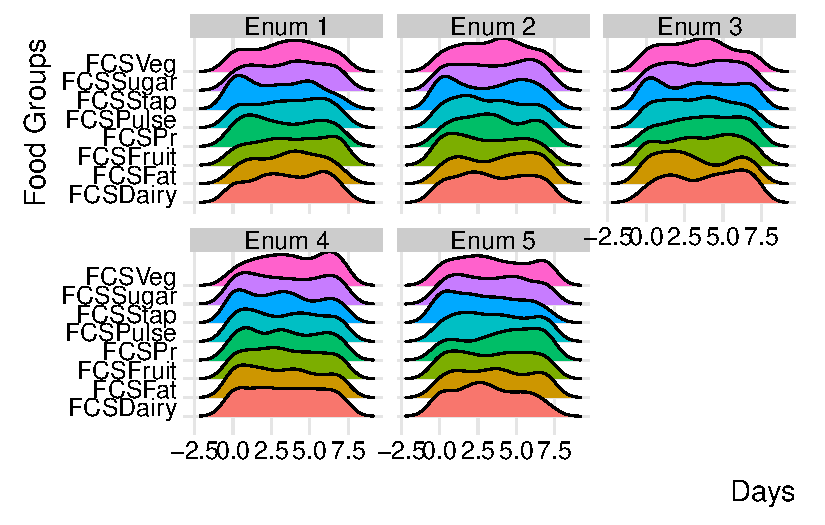
\includegraphics{chapter_two_files/figure-pdf/unnamed-chunk-10-1.pdf}

}

\end{figure}

By carefully examining and interpreting the ridge chart, you can gain
valuable insights into the distributions and flag any inconsistency for
validation and review during data collection. in the below chart, we'll
group the reduced coping strategies at area office level.

\begin{Shaded}
\begin{Highlighting}[]
\NormalTok{(}\FunctionTok{plot\_ridge\_distribution}\NormalTok{(survey\_df, }\AttributeTok{numeric\_cols =} \FunctionTok{c}\NormalTok{(}\StringTok{"rCSILessQlty"}\NormalTok{, }\StringTok{"rCSIBorrow"}\NormalTok{, }\StringTok{"rCSIMealSize"}\NormalTok{, }\StringTok{"rCSIMealAdult"}\NormalTok{, }\StringTok{"rCSIMealNb"}\NormalTok{),}
                         \AttributeTok{name\_groups =} \StringTok{"Food Coping Strategy"}\NormalTok{, }\AttributeTok{name\_units =} \StringTok{"Days"}\NormalTok{, }\AttributeTok{grouping =} \StringTok{"EnuName"}\NormalTok{))}
\end{Highlighting}
\end{Shaded}

\begin{figure}[H]

{\centering 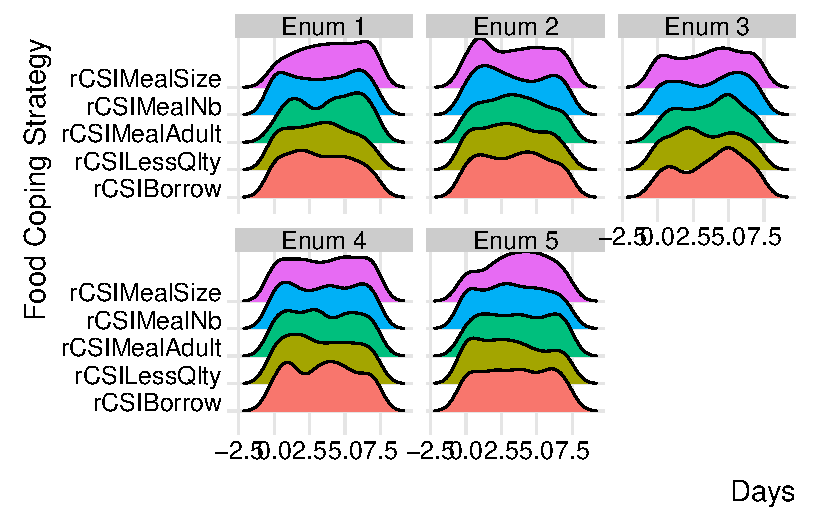
\includegraphics{chapter_two_files/figure-pdf/unnamed-chunk-11-1.pdf}

}

\end{figure}

similarly, you can group distributions at field monitor level to gain
more insight at the consistency of reported distributions across
different monitors.

\begin{Shaded}
\begin{Highlighting}[]
\NormalTok{(}\FunctionTok{plot\_ridge\_distribution}\NormalTok{(survey\_df, }\AttributeTok{numeric\_cols =} \FunctionTok{c}\NormalTok{(}\StringTok{"rCSILessQlty"}\NormalTok{, }\StringTok{"rCSIBorrow"}\NormalTok{, }\StringTok{"rCSIMealSize"}\NormalTok{, }\StringTok{"rCSIMealAdult"}\NormalTok{, }\StringTok{"rCSIMealNb"}\NormalTok{),}
                         \AttributeTok{name\_groups =} \StringTok{"Food Coping Strategy"}\NormalTok{, }\AttributeTok{name\_units =} \StringTok{"Days"}\NormalTok{, }\AttributeTok{grouping =} \StringTok{"EnuName"}\NormalTok{))}
\end{Highlighting}
\end{Shaded}

\begin{figure}[H]

{\centering 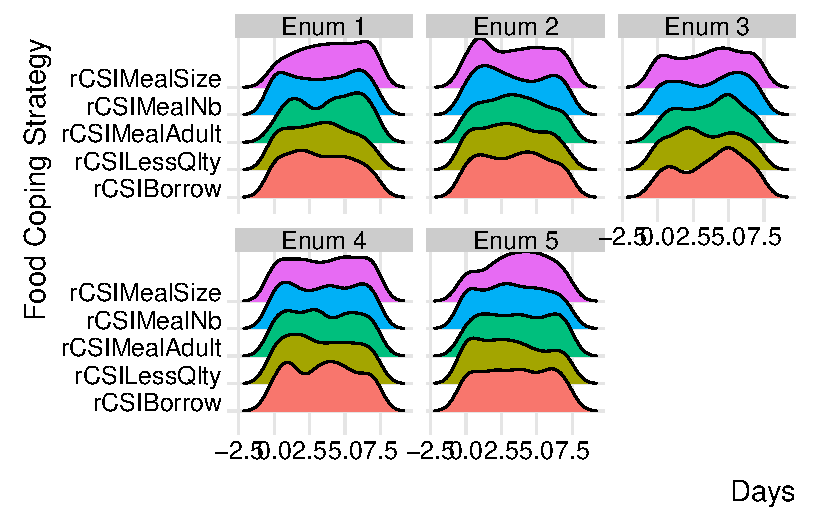
\includegraphics{chapter_two_files/figure-pdf/unnamed-chunk-12-1.pdf}

}

\end{figure}

\hypertarget{apply-cleaning-log}{%
\section{Apply Cleaning Log}\label{apply-cleaning-log}}

\hypertarget{spatial-verification}{%
\section{Spatial Verification}\label{spatial-verification}}

\bookmarksetup{startatroot}

\hypertarget{calculating-indicators}{%
\chapter{Calculating Indicators}\label{calculating-indicators}}

\begin{Shaded}
\begin{Highlighting}[]
\FunctionTok{library}\NormalTok{(tidyverse)}
\FunctionTok{library}\NormalTok{(tidyr)}
\FunctionTok{library}\NormalTok{(readxl)}
\FunctionTok{library}\NormalTok{(labelled)}
\FunctionTok{library}\NormalTok{(expss)}

\NormalTok{survey\_df3 }\OtherTok{\textless{}{-}} \FunctionTok{read\_excel}\NormalTok{(}\StringTok{"input/MoDa\_Data\_2025{-}03{-}13.xlsx"}\NormalTok{)}
\end{Highlighting}
\end{Shaded}

\hypertarget{food-security-essential-needs}{%
\section{Food Security \& Essential
Needs}\label{food-security-essential-needs}}

\hypertarget{food-consumption-score-fcs}{%
\subsection{Food Consumption Score
(FCS)}\label{food-consumption-score-fcs}}

The food consumption score (FCS) indicator is a composite score based on
households' dietary diversity, food consumption frequency and relative
nutritional value of different food groups. The FCS aggregated
household-level food consumption data, in terms of frequency over the
previous seven days and weights data accordingly to the relative value
of the consumed food groups.

Cut-off thresholds are applied to the FCS to classify households into
three groups: poor, borderline or acceptable food consumption.

\begin{Shaded}
\begin{Highlighting}[]
\CommentTok{\# compute FCS function}
\NormalTok{compute\_fcs }\OtherTok{\textless{}{-}} \ControlFlowTok{function}\NormalTok{(df,}
\NormalTok{                        FCSStap,}
\NormalTok{                        FCSPulse,}
\NormalTok{                        FCSPr,}
\NormalTok{                        FCSVeg,}
\NormalTok{                        FCSFruit,}
\NormalTok{                        FCSDairy,}
\NormalTok{                        FCSFat,}
\NormalTok{                        FCSSugar,}
\NormalTok{                        cutoff)\{}
  
  \CommentTok{\# check food consumption variables}
\NormalTok{  fcs\_cols }\OtherTok{\textless{}{-}} \FunctionTok{c}\NormalTok{(FCSStap, FCSPulse, FCSPr, FCSVeg, FCSFruit, FCSDairy, FCSFat, FCSSugar)}
  
\NormalTok{  check\_df }\OtherTok{\textless{}{-}}\NormalTok{ df }\SpecialCharTok{\%\textgreater{}\%}\NormalTok{ dplyr}\SpecialCharTok{::}\FunctionTok{filter}\NormalTok{(}\FunctionTok{pmax}\NormalTok{(}\SpecialCharTok{!!!}\FunctionTok{syms}\NormalTok{(fcs\_cols), }\AttributeTok{na.rm =}\NormalTok{ T) }\SpecialCharTok{==} \FunctionTok{pmin}\NormalTok{(}\SpecialCharTok{!!!}\FunctionTok{syms}\NormalTok{(fcs\_cols), }\AttributeTok{na.rm =}\NormalTok{ T))}
  
  \CommentTok{\# check cutoff argument}
  \ControlFlowTok{if}\NormalTok{(}\SpecialCharTok{!}\NormalTok{(cutoff }\SpecialCharTok{\%in\%} \FunctionTok{c}\NormalTok{(}\StringTok{"Cat28"}\NormalTok{, }\StringTok{"Cat21"}\NormalTok{))) \{}
    \FunctionTok{stop}\NormalTok{(glue}\SpecialCharTok{::}\FunctionTok{glue}\NormalTok{(}\StringTok{"\textasciigrave{}cutoff\textasciigrave{} must be one of: \textasciigrave{}Cat28\textasciigrave{} or \textasciigrave{}Cat21\textasciigrave{}, not \{cutoff\}."}\NormalTok{))}
\NormalTok{  \}}
  
  \ControlFlowTok{if}\NormalTok{(}\SpecialCharTok{!}\FunctionTok{is.null}\NormalTok{(FCSStap) }\SpecialCharTok{\&\&} \SpecialCharTok{!}\FunctionTok{is.null}\NormalTok{(FCSPulse)) \{}
\NormalTok{    df }\OtherTok{\textless{}{-}}\NormalTok{ df }\SpecialCharTok{\%\textgreater{}\%}
      \FunctionTok{mutate}\NormalTok{(}\AttributeTok{FCS =}\NormalTok{ (FCSStap }\SpecialCharTok{*} \DecValTok{2}\NormalTok{) }\SpecialCharTok{+}\NormalTok{ (FCSPulse }\SpecialCharTok{*} \DecValTok{3}\NormalTok{) }\SpecialCharTok{+}\NormalTok{ (FCSPr }\SpecialCharTok{*} \DecValTok{4}\NormalTok{) }\SpecialCharTok{+}
\NormalTok{               (FCSDairy }\SpecialCharTok{*} \DecValTok{4}\NormalTok{) }\SpecialCharTok{+}\NormalTok{ FCSVeg }\SpecialCharTok{+}\NormalTok{ FCSFruit }\SpecialCharTok{+}\NormalTok{ (FCSFat }\SpecialCharTok{*} \FloatTok{0.5}\NormalTok{) }\SpecialCharTok{+}
\NormalTok{               (FCSSugar }\SpecialCharTok{*} \FloatTok{0.5}\NormalTok{))}
    
\NormalTok{    df }\OtherTok{\textless{}{-}}\NormalTok{ df }\SpecialCharTok{\%\textgreater{}\%}
      \FunctionTok{mutate}\NormalTok{(}
        \AttributeTok{FCSCat =} \FunctionTok{case\_when}\NormalTok{(}
\NormalTok{          cutoff }\SpecialCharTok{==} \StringTok{"Cat28"} \SpecialCharTok{\textasciitilde{}} \FunctionTok{case\_when}\NormalTok{(}
\NormalTok{            FCS }\SpecialCharTok{\textless{}=} \DecValTok{28} \SpecialCharTok{\textasciitilde{}} \DecValTok{1}\NormalTok{,}
            \FunctionTok{between}\NormalTok{(FCS, }\FloatTok{28.5}\NormalTok{, }\DecValTok{42}\NormalTok{) }\SpecialCharTok{\textasciitilde{}} \DecValTok{2}\NormalTok{,}
            \ConstantTok{TRUE} \SpecialCharTok{\textasciitilde{}} \DecValTok{3}
\NormalTok{          ),}
\NormalTok{          cutoff }\SpecialCharTok{==} \StringTok{"Cat21"} \SpecialCharTok{\textasciitilde{}} \FunctionTok{case\_when}\NormalTok{(}
\NormalTok{            FCS }\SpecialCharTok{\textless{}=} \DecValTok{21} \SpecialCharTok{\textasciitilde{}} \DecValTok{1}\NormalTok{,}
            \FunctionTok{between}\NormalTok{(FCS, }\FloatTok{21.5}\NormalTok{, }\DecValTok{35}\NormalTok{) }\SpecialCharTok{\textasciitilde{}} \DecValTok{2}\NormalTok{,}
            \ConstantTok{TRUE} \SpecialCharTok{\textasciitilde{}} \DecValTok{3}
\NormalTok{          )}
\NormalTok{        )}
\NormalTok{      )}
\NormalTok{  \}}
  
\NormalTok{\}}
\end{Highlighting}
\end{Shaded}

\begin{Shaded}
\begin{Highlighting}[]
\NormalTok{survey\_df3 }\OtherTok{\textless{}{-}} \FunctionTok{compute\_fcs}\NormalTok{(}\AttributeTok{df =}\NormalTok{ survey\_df3,}
                          \AttributeTok{FCSStap =} \StringTok{"FCSStap"}\NormalTok{,}
                          \AttributeTok{FCSPr =} \StringTok{"FCSPr"}\NormalTok{,}
                          \AttributeTok{FCSPulse =} \StringTok{"FCSPulse"}\NormalTok{,}
                          \AttributeTok{FCSVeg =} \StringTok{"FCSVeg"}\NormalTok{,}
                          \AttributeTok{FCSFruit =} \StringTok{"FCSFruit"}\NormalTok{,}
                          \AttributeTok{FCSDairy =} \StringTok{"FCSDairy"}\NormalTok{,}
                          \AttributeTok{FCSFat =} \StringTok{"FCSFat"}\NormalTok{,}
                          \AttributeTok{FCSSugar =} \StringTok{"FCSSugar"}\NormalTok{,}
                          \AttributeTok{cutoff =} \StringTok{"Cat21"}\NormalTok{)}
\end{Highlighting}
\end{Shaded}

\begin{Shaded}
\begin{Highlighting}[]
\NormalTok{knitr}\SpecialCharTok{::}\FunctionTok{kable}\NormalTok{(}
  \FunctionTok{head}\NormalTok{(survey\_df3[, }\FunctionTok{c}\NormalTok{(}\StringTok{"ADMIN1Name"}\NormalTok{, }\StringTok{"FCS"}\NormalTok{, }\StringTok{"FCSCat"}\NormalTok{)], }\DecValTok{5}\NormalTok{),}
  \AttributeTok{caption =} \StringTok{"Survey Tracking Table"}\NormalTok{,}
  \AttributeTok{booktabs =} \ConstantTok{TRUE}
\NormalTok{)}
\end{Highlighting}
\end{Shaded}

\begin{longtable}[]{@{}lrr@{}}
\caption{Survey Tracking Table}\tabularnewline
\toprule\noalign{}
ADMIN1Name & FCS & FCSCat \\
\midrule\noalign{}
\endfirsthead
\toprule\noalign{}
ADMIN1Name & FCS & FCSCat \\
\midrule\noalign{}
\endhead
\bottomrule\noalign{}
\endlastfoot
Admin 3 & 63.5 & 3 \\
Admin 1 & 68.5 & 3 \\
Admin 1 & 57.5 & 3 \\
Admin 1 & 40.5 & 3 \\
Admin 3 & 38.0 & 3 \\
\end{longtable}

\hypertarget{food-consumption-score-nutrition-fcs-n}{%
\subsection{Food Consumption Score Nutrition
(FCS-N)}\label{food-consumption-score-nutrition-fcs-n}}

FCS-N is a measure of household's adequacy of key macro and
micronutrients-rich food groups. In order to assess nutrient inadequacy,
FCS-N looks at the frequencies of consumption of protein-rich, Hem Iron
and Vitamin A-rich foods over the 7 days prior to the interview.

\begin{Shaded}
\begin{Highlighting}[]
\CommentTok{\# first record NA values to 0}
\NormalTok{survey\_df3}\SpecialCharTok{$}\NormalTok{FCSNPrMeatF[}\FunctionTok{is.na}\NormalTok{(survey\_df3}\SpecialCharTok{$}\NormalTok{FCSNPrMeatF)] }\OtherTok{\textless{}{-}} \DecValTok{0}
\NormalTok{survey\_df3}\SpecialCharTok{$}\NormalTok{FCSNPrMeatO[}\FunctionTok{is.na}\NormalTok{(survey\_df3}\SpecialCharTok{$}\NormalTok{FCSNPrMeatO)] }\OtherTok{\textless{}{-}} \DecValTok{0}
\NormalTok{survey\_df3}\SpecialCharTok{$}\NormalTok{FCSNPrFish[}\FunctionTok{is.na}\NormalTok{(survey\_df3}\SpecialCharTok{$}\NormalTok{FCSNPrFish)] }\OtherTok{\textless{}{-}} \DecValTok{0}
\NormalTok{survey\_df3}\SpecialCharTok{$}\NormalTok{FCSNPrEggs[}\FunctionTok{is.na}\NormalTok{(survey\_df3}\SpecialCharTok{$}\NormalTok{FCSNPrEggs)] }\OtherTok{\textless{}{-}} \DecValTok{0}
\NormalTok{survey\_df3}\SpecialCharTok{$}\NormalTok{FCSVeg[}\FunctionTok{is.na}\NormalTok{(survey\_df3}\SpecialCharTok{$}\NormalTok{FCSVeg)] }\OtherTok{\textless{}{-}} \DecValTok{0}
\NormalTok{survey\_df3}\SpecialCharTok{$}\NormalTok{FCSNVegGre[}\FunctionTok{is.na}\NormalTok{(survey\_df3}\SpecialCharTok{$}\NormalTok{FCSNVegGre)] }\OtherTok{\textless{}{-}} \DecValTok{0}
\NormalTok{survey\_df3}\SpecialCharTok{$}\NormalTok{FCSFruit[}\FunctionTok{is.na}\NormalTok{(survey\_df3}\SpecialCharTok{$}\NormalTok{FCSFruit)] }\OtherTok{\textless{}{-}} \DecValTok{0}

\CommentTok{\# Compute aggregates of key micronutrient consumption}
\DocumentationTok{\#\# Vitamin A{-}Rich Foods}
\NormalTok{survey\_df3 }\OtherTok{\textless{}{-}}\NormalTok{ survey\_df3 }\SpecialCharTok{\%\textgreater{}\%} \FunctionTok{mutate}\NormalTok{(}\AttributeTok{FGVitA =}\NormalTok{ FCSDairy }\SpecialCharTok{+}\NormalTok{FCSNPrMeatO }\SpecialCharTok{+}\NormalTok{FCSNPrEggs }\SpecialCharTok{+}
\NormalTok{                                  FCSNVegOrg }\SpecialCharTok{+}\NormalTok{FCSNVegGre }\SpecialCharTok{+}\NormalTok{FCSNFruiOrg)}
\FunctionTok{var\_label}\NormalTok{(survey\_df3}\SpecialCharTok{$}\NormalTok{FGVitA) }\OtherTok{\textless{}{-}} \StringTok{"Consumption of vitamin A{-}rich foods"}

\DocumentationTok{\#\# Protein{-}Rich Foods}
\NormalTok{survey\_df3 }\OtherTok{\textless{}{-}}\NormalTok{ survey\_df3 }\SpecialCharTok{\%\textgreater{}\%} \FunctionTok{mutate}\NormalTok{(}\AttributeTok{FGProtein =}\NormalTok{ FCSPr }\SpecialCharTok{+}\NormalTok{FCSDairy }\SpecialCharTok{+}\NormalTok{FCSNPrMeatF }\SpecialCharTok{+}
\NormalTok{                                  FCSNPrMeatO }\SpecialCharTok{+}\NormalTok{FCSNPrFish }\SpecialCharTok{+}\NormalTok{FCSNVegOrg)}
\FunctionTok{var\_label}\NormalTok{(survey\_df3}\SpecialCharTok{$}\NormalTok{FGProtein) }\OtherTok{\textless{}{-}} \StringTok{"Consumption of protein{-}rich foods"}

\DocumentationTok{\#\# Iron{-}Rich Foods}
\NormalTok{survey\_df3 }\OtherTok{\textless{}{-}}\NormalTok{ survey\_df3 }\SpecialCharTok{\%\textgreater{}\%} \FunctionTok{mutate}\NormalTok{(}\AttributeTok{FGHIron =}\NormalTok{ FCSNPrMeatF }\SpecialCharTok{+}\NormalTok{FCSNPrMeatO }\SpecialCharTok{+}\NormalTok{FCSNPrFish)}
\FunctionTok{var\_label}\NormalTok{(survey\_df3}\SpecialCharTok{$}\NormalTok{FGHIron) }\OtherTok{\textless{}{-}} \StringTok{"Consumption of heme iron{-}rich foods"}

\DocumentationTok{\#\# recode into nutritious groups}
\NormalTok{survey\_df3 }\OtherTok{\textless{}{-}}\NormalTok{ survey\_df3 }\SpecialCharTok{\%\textgreater{}\%} \FunctionTok{mutate}\NormalTok{(}\AttributeTok{FGVitACat =} \FunctionTok{case\_when}\NormalTok{(FGVitA }\SpecialCharTok{==} \DecValTok{0} \SpecialCharTok{\textasciitilde{}} \DecValTok{1}\NormalTok{,}
                                                          \FunctionTok{between}\NormalTok{(FGVitA,}\DecValTok{1}\NormalTok{,}\DecValTok{6}\NormalTok{) }\SpecialCharTok{\textasciitilde{}} \DecValTok{2}\NormalTok{, }
\NormalTok{                                                          FGVitA }\SpecialCharTok{\textgreater{}=} \DecValTok{7} \SpecialCharTok{\textasciitilde{}} \DecValTok{3}\NormalTok{),}
                                    \AttributeTok{FGProteinCat =} \FunctionTok{case\_when}\NormalTok{(FGProtein }\SpecialCharTok{==} \DecValTok{0} \SpecialCharTok{\textasciitilde{}} \DecValTok{1}\NormalTok{, }
                                                             \FunctionTok{between}\NormalTok{(FGProtein,}\DecValTok{1}\NormalTok{,}\DecValTok{6}\NormalTok{) }\SpecialCharTok{\textasciitilde{}} \DecValTok{2}\NormalTok{,}
\NormalTok{                                                             FGProtein }\SpecialCharTok{\textgreater{}=} \DecValTok{7} \SpecialCharTok{\textasciitilde{}} \DecValTok{3}\NormalTok{),}
                                    \AttributeTok{FGHIronCat =} \FunctionTok{case\_when}\NormalTok{(FGHIron }\SpecialCharTok{==} \DecValTok{0} \SpecialCharTok{\textasciitilde{}} \DecValTok{1}\NormalTok{,}
                                                           \FunctionTok{between}\NormalTok{(FGHIron,}\DecValTok{1}\NormalTok{,}\DecValTok{6}\NormalTok{) }\SpecialCharTok{\textasciitilde{}} \DecValTok{2}\NormalTok{,}
\NormalTok{                                                           FGHIron }\SpecialCharTok{\textgreater{}=} \DecValTok{7} \SpecialCharTok{\textasciitilde{}} \DecValTok{3}\NormalTok{))}

\CommentTok{\# define variables labels and properties for FGVitACat FGProteinCat FGHIronCat}
\NormalTok{survey\_df3 }\OtherTok{\textless{}{-}}\NormalTok{ survey\_df3 }\SpecialCharTok{\%\textgreater{}\%}
  \FunctionTok{mutate}\NormalTok{(}\FunctionTok{across}\NormalTok{(}\FunctionTok{c}\NormalTok{(FGVitACat, FGProteinCat, FGHIronCat), }
                \SpecialCharTok{\textasciitilde{}}\FunctionTok{labelled}\NormalTok{(., }\AttributeTok{labels =} \FunctionTok{c}\NormalTok{(}
                  \StringTok{"Never consumed"} \OtherTok{=} \DecValTok{1}\NormalTok{,}
                  \StringTok{"Consumed sometimes"} \OtherTok{=} \DecValTok{2}\NormalTok{,}
                  \StringTok{"Consumed at least 7 times"} \OtherTok{=} \DecValTok{3}
\NormalTok{                ))))}

\NormalTok{survey\_df3 }\OtherTok{\textless{}{-}}\NormalTok{ survey\_df3 }\SpecialCharTok{\%\textgreater{}\%}
  \FunctionTok{mutate}\NormalTok{(}\FunctionTok{across}\NormalTok{(}\FunctionTok{c}\NormalTok{(FGVitACat, FGProteinCat, FGHIronCat),}
                \SpecialCharTok{\textasciitilde{}}\FunctionTok{factor}\NormalTok{(., }\AttributeTok{levels =} \FunctionTok{c}\NormalTok{(}\DecValTok{1}\NormalTok{, }\DecValTok{2}\NormalTok{, }\DecValTok{3}\NormalTok{),}
                        \AttributeTok{labels =} \FunctionTok{c}\NormalTok{(}\StringTok{"Never consumed"}\NormalTok{, }\StringTok{"Consumed sometimes"}\NormalTok{, }
                                   \StringTok{"Consumed at least 7 times"}\NormalTok{))))}
\end{Highlighting}
\end{Shaded}

\begin{Shaded}
\begin{Highlighting}[]
\NormalTok{knitr}\SpecialCharTok{::}\FunctionTok{kable}\NormalTok{(}
  \FunctionTok{head}\NormalTok{(survey\_df3[, }\FunctionTok{c}\NormalTok{(}\StringTok{"ADMIN1Name"}\NormalTok{, }\StringTok{"FGVitACat"}\NormalTok{, }\StringTok{"FGProteinCat"}\NormalTok{, }\StringTok{"FGHIronCat"}\NormalTok{)], }\DecValTok{5}\NormalTok{),}
  \AttributeTok{caption =} \StringTok{"FCSN table"}\NormalTok{,}
  \AttributeTok{booktabs =} \ConstantTok{TRUE}
\NormalTok{)}
\end{Highlighting}
\end{Shaded}

\begin{longtable}[]{@{}
  >{\raggedright\arraybackslash}p{(\columnwidth - 6\tabcolsep) * \real{0.1236}}
  >{\raggedright\arraybackslash}p{(\columnwidth - 6\tabcolsep) * \real{0.2921}}
  >{\raggedright\arraybackslash}p{(\columnwidth - 6\tabcolsep) * \real{0.2921}}
  >{\raggedright\arraybackslash}p{(\columnwidth - 6\tabcolsep) * \real{0.2921}}@{}}
\caption{FCSN table}\tabularnewline
\toprule\noalign{}
\begin{minipage}[b]{\linewidth}\raggedright
ADMIN1Name
\end{minipage} & \begin{minipage}[b]{\linewidth}\raggedright
FGVitACat
\end{minipage} & \begin{minipage}[b]{\linewidth}\raggedright
FGProteinCat
\end{minipage} & \begin{minipage}[b]{\linewidth}\raggedright
FGHIronCat
\end{minipage} \\
\midrule\noalign{}
\endfirsthead
\toprule\noalign{}
\begin{minipage}[b]{\linewidth}\raggedright
ADMIN1Name
\end{minipage} & \begin{minipage}[b]{\linewidth}\raggedright
FGVitACat
\end{minipage} & \begin{minipage}[b]{\linewidth}\raggedright
FGProteinCat
\end{minipage} & \begin{minipage}[b]{\linewidth}\raggedright
FGHIronCat
\end{minipage} \\
\midrule\noalign{}
\endhead
\bottomrule\noalign{}
\endlastfoot
Admin 3 & Consumed at least 7 times & Consumed at least 7 times &
Consumed sometimes \\
Admin 1 & Consumed at least 7 times & Consumed at least 7 times &
Consumed at least 7 times \\
Admin 1 & Consumed at least 7 times & Consumed at least 7 times &
Consumed at least 7 times \\
Admin 1 & Consumed at least 7 times & Consumed at least 7 times &
Consumed at least 7 times \\
Admin 3 & Consumed at least 7 times & Consumed at least 7 times &
Consumed at least 7 times \\
\end{longtable}

\hypertarget{household-dietary-diversity-hdds}{%
\subsection{Household Dietary Diversity
(HDDs)}\label{household-dietary-diversity-hdds}}

\begin{Shaded}
\begin{Highlighting}[]
\CommentTok{\# compute HHDs}
\NormalTok{compute\_hdds }\OtherTok{\textless{}{-}} \ControlFlowTok{function}\NormalTok{(df,}
\NormalTok{                         HDDSStapCer,}
\NormalTok{                         HDDSStapRoot,}
\NormalTok{                         HDDSPulse,}
\NormalTok{                         HDDSDairy,}
\NormalTok{                         HDDSPrMeat,}
\NormalTok{                         HDDSPrFish,}
\NormalTok{                         HDDSPrEggs,}
\NormalTok{                         HDDSVeg,}
\NormalTok{                         HDDSFruit,}
\NormalTok{                         HDDSFat,}
\NormalTok{                         HDDSSugar,}
\NormalTok{                         HDDSCond) \{}
  
  \CommentTok{\# Convert relevant columns to numeric}
\NormalTok{  df }\OtherTok{\textless{}{-}}\NormalTok{ df }\SpecialCharTok{\%\textgreater{}\%}
    \FunctionTok{mutate}\NormalTok{(}\FunctionTok{across}\NormalTok{(}
      \AttributeTok{.cols =} \FunctionTok{all\_of}\NormalTok{(}\FunctionTok{c}\NormalTok{(HDDSStapCer, HDDSStapRoot, HDDSPulse, HDDSDairy,}
\NormalTok{                       HDDSPrMeat, HDDSPrFish, HDDSPrEggs, HDDSVeg,}
\NormalTok{                       HDDSFruit, HDDSFat, HDDSSugar, HDDSCond)),}
      \AttributeTok{.fns =} \SpecialCharTok{\textasciitilde{}} \FunctionTok{as.numeric}\NormalTok{(.),}
      \AttributeTok{.names =} \StringTok{"num\_\{.col\}"}
\NormalTok{    ))}
  
  \CommentTok{\# Compute HDDS using the numeric versions}
\NormalTok{  df }\OtherTok{\textless{}{-}}\NormalTok{ df }\SpecialCharTok{\%\textgreater{}\%}
    \FunctionTok{rowwise}\NormalTok{() }\SpecialCharTok{\%\textgreater{}\%}
    \FunctionTok{mutate}\NormalTok{(}\AttributeTok{HDDS =} \FunctionTok{sum}\NormalTok{(}\FunctionTok{c\_across}\NormalTok{(}\FunctionTok{starts\_with}\NormalTok{(}\StringTok{"num\_"}\NormalTok{)), }\AttributeTok{na.rm =} \ConstantTok{TRUE}\NormalTok{)) }\SpecialCharTok{\%\textgreater{}\%}
    \FunctionTok{ungroup}\NormalTok{()}
  
  \CommentTok{\# Categorize HDDS}
\NormalTok{  df }\OtherTok{\textless{}{-}}\NormalTok{ df }\SpecialCharTok{\%\textgreater{}\%}
    \FunctionTok{mutate}\NormalTok{(}\AttributeTok{HDDSCat\_IPC =} \FunctionTok{case\_when}\NormalTok{(}
\NormalTok{      HDDS }\SpecialCharTok{\textless{}=} \DecValTok{2} \SpecialCharTok{\textasciitilde{}} \DecValTok{1}\NormalTok{,}
\NormalTok{      HDDS }\SpecialCharTok{\textgreater{}=} \DecValTok{3} \SpecialCharTok{\&}\NormalTok{ HDDS }\SpecialCharTok{\textless{}=} \DecValTok{4} \SpecialCharTok{\textasciitilde{}} \DecValTok{2}\NormalTok{,}
\NormalTok{      HDDS }\SpecialCharTok{==} \DecValTok{5} \SpecialCharTok{\textasciitilde{}} \DecValTok{3}\NormalTok{,}
\NormalTok{      HDDS }\SpecialCharTok{\textgreater{}=} \DecValTok{6} \SpecialCharTok{\textasciitilde{}} \DecValTok{4}
\NormalTok{    ))}
  
  \FunctionTok{return}\NormalTok{(df)}
\NormalTok{\}}
\end{Highlighting}
\end{Shaded}

\begin{Shaded}
\begin{Highlighting}[]
\NormalTok{survey\_df3 }\OtherTok{\textless{}{-}} \FunctionTok{compute\_hdds}\NormalTok{(}\AttributeTok{df =}\NormalTok{ survey\_df3,}
                           \AttributeTok{HDDSStapCer =} \StringTok{"HDDSStapCer"}\NormalTok{,}
                           \AttributeTok{HDDSStapRoot =} \StringTok{"HDDSStapRoot"}\NormalTok{,}
                           \AttributeTok{HDDSPulse =} \StringTok{"HDDSPulse"}\NormalTok{,}
                           \AttributeTok{HDDSDairy =} \StringTok{"HDDSDairy"}\NormalTok{,}
                           \AttributeTok{HDDSPrMeat =} \StringTok{"HDDSPrMeat"}\NormalTok{,}
                           \AttributeTok{HDDSPrFish =} \StringTok{"HDDSPrFish"}\NormalTok{,}
                           \AttributeTok{HDDSPrEggs =} \StringTok{"HDDSPrEggs"}\NormalTok{,}
                           \AttributeTok{HDDSVeg =} \StringTok{"HDDSVeg"}\NormalTok{,}
                           \AttributeTok{HDDSFruit =} \StringTok{"HDDSFruit"}\NormalTok{,}
                           \AttributeTok{HDDSFat =} \StringTok{"HDDSFat"}\NormalTok{,}
                           \AttributeTok{HDDSSugar =} \StringTok{"HDDSSugar"}\NormalTok{,}
                           \AttributeTok{HDDSCond =} \StringTok{"HDDSCond"}\NormalTok{)}
\end{Highlighting}
\end{Shaded}

\begin{Shaded}
\begin{Highlighting}[]
\NormalTok{knitr}\SpecialCharTok{::}\FunctionTok{kable}\NormalTok{(}
  \FunctionTok{head}\NormalTok{(survey\_df3[, }\FunctionTok{c}\NormalTok{(}\StringTok{"ADMIN1Name"}\NormalTok{, }\StringTok{"HDDS"}\NormalTok{, }\StringTok{"HDDSCat\_IPC"}\NormalTok{)], }\DecValTok{5}\NormalTok{),}
  \AttributeTok{caption =} \StringTok{"Survey Tracking Table"}\NormalTok{,}
  \AttributeTok{booktabs =} \ConstantTok{TRUE}
\NormalTok{)}
\end{Highlighting}
\end{Shaded}

\begin{longtable}[]{@{}lrr@{}}
\caption{Survey Tracking Table}\tabularnewline
\toprule\noalign{}
ADMIN1Name & HDDS & HDDSCat\_IPC \\
\midrule\noalign{}
\endfirsthead
\toprule\noalign{}
ADMIN1Name & HDDS & HDDSCat\_IPC \\
\midrule\noalign{}
\endhead
\bottomrule\noalign{}
\endlastfoot
Admin 3 & 6 & 4 \\
Admin 1 & 4 & 2 \\
Admin 1 & 7 & 4 \\
Admin 1 & 6 & 4 \\
Admin 3 & 7 & 4 \\
\end{longtable}

\hypertarget{reduced-coping-strategies-rcsi}{%
\subsection{Reduced Coping Strategies
(rCSI)}\label{reduced-coping-strategies-rcsi}}

The Reduced Coping Strategy Index (rCSI), also called CSI food, is used
to assess the level of stress3 faced by a household due to a food
shortage. It is measured by combining the frequency and severity of the
food consumption based strategies households are engaging in. It is
calculated using the five standard strategies using a 7-day recall
period.

\begin{Shaded}
\begin{Highlighting}[]
\NormalTok{survey\_df3 }\OtherTok{\textless{}{-}}\NormalTok{ survey\_df3 }\SpecialCharTok{\%\textgreater{}\%} 
  \FunctionTok{mutate}\NormalTok{(}\AttributeTok{rCSI =}\NormalTok{ rCSILessQlty }\SpecialCharTok{+}\NormalTok{ (rCSIBorrow }\SpecialCharTok{*} \DecValTok{2}\NormalTok{) }\SpecialCharTok{+}\NormalTok{ rCSIMealSize }\SpecialCharTok{+}\NormalTok{ (rCSIMealAdult }\SpecialCharTok{*} \DecValTok{3}\NormalTok{) }\SpecialCharTok{+}\NormalTok{ rCSIMealNb)}
\end{Highlighting}
\end{Shaded}

\begin{Shaded}
\begin{Highlighting}[]
\NormalTok{knitr}\SpecialCharTok{::}\FunctionTok{kable}\NormalTok{(}
  \FunctionTok{head}\NormalTok{(survey\_df3[, }\FunctionTok{c}\NormalTok{(}\StringTok{"ADMIN1Name"}\NormalTok{, }\StringTok{"rCSI"}\NormalTok{)], }\DecValTok{5}\NormalTok{),}
  \AttributeTok{caption =} \StringTok{"rCSI table"}\NormalTok{,}
  \AttributeTok{booktabs =} \ConstantTok{TRUE}
\NormalTok{)}
\end{Highlighting}
\end{Shaded}

\begin{longtable}[]{@{}lr@{}}
\caption{rCSI table}\tabularnewline
\toprule\noalign{}
ADMIN1Name & rCSI \\
\midrule\noalign{}
\endfirsthead
\toprule\noalign{}
ADMIN1Name & rCSI \\
\midrule\noalign{}
\endhead
\bottomrule\noalign{}
\endlastfoot
Admin 3 & 14 \\
Admin 1 & 39 \\
Admin 1 & 20 \\
Admin 1 & 13 \\
Admin 3 & 16 \\
\end{longtable}

\hypertarget{livelihood-coping-strategies-lcs-fs}{%
\subsection{Livelihood Coping Strategies
(LCS-FS)}\label{livelihood-coping-strategies-lcs-fs}}

The livelihoods-based coping strategies module is used to better
understand longer-term coping capacity of households. For each country,
the module must be adapted to suit each country's context and poor
people's living conditions.

\begin{Shaded}
\begin{Highlighting}[]
\NormalTok{survey\_df3 }\OtherTok{\textless{}{-}}\NormalTok{ survey\_df3 }\SpecialCharTok{\%\textgreater{}\%} 
  \FunctionTok{mutate}\NormalTok{(}
    \CommentTok{\# stress}
    \AttributeTok{stress\_coping\_FS =} \FunctionTok{case\_when}\NormalTok{(}
\NormalTok{      Lcs\_stress\_DomAsset }\SpecialCharTok{==} \DecValTok{20} \SpecialCharTok{|}\NormalTok{  Lcs\_stress\_DomAsset }\SpecialCharTok{==} \DecValTok{30} \SpecialCharTok{\textasciitilde{}} \DecValTok{1}\NormalTok{,}
\NormalTok{      Lcs\_stress\_Saving }\SpecialCharTok{==} \DecValTok{20} \SpecialCharTok{|}\NormalTok{ Lcs\_stress\_Saving }\SpecialCharTok{==} \DecValTok{30} \SpecialCharTok{\textasciitilde{}} \DecValTok{1}\NormalTok{,}
\NormalTok{      Lcs\_stress\_BorrowCash }\SpecialCharTok{==} \DecValTok{20} \SpecialCharTok{|}\NormalTok{ Lcs\_stress\_BorrowCash }\SpecialCharTok{==} \DecValTok{30} \SpecialCharTok{\textasciitilde{}} \DecValTok{1}\NormalTok{,}
\NormalTok{      Lcs\_stress\_Edu }\SpecialCharTok{==} \DecValTok{20} \SpecialCharTok{|}\NormalTok{ Lcs\_stress\_Edu }\SpecialCharTok{==} \DecValTok{30} \SpecialCharTok{\textasciitilde{}}\DecValTok{1}\NormalTok{,}
      \ConstantTok{TRUE} \SpecialCharTok{\textasciitilde{}} \DecValTok{0}
\NormalTok{    ),}
    
    \CommentTok{\# crisis}
    \AttributeTok{crisis\_coping\_FS =} \FunctionTok{case\_when}\NormalTok{(}
\NormalTok{      Lcs\_crisis\_Health }\SpecialCharTok{==} \DecValTok{20} \SpecialCharTok{|}\NormalTok{  Lcs\_crisis\_Health }\SpecialCharTok{==} \DecValTok{30} \SpecialCharTok{\textasciitilde{}} \DecValTok{1}\NormalTok{,}
\NormalTok{      Lcs\_crisis\_OutSchool }\SpecialCharTok{==} \DecValTok{20} \SpecialCharTok{|}\NormalTok{ Lcs\_crisis\_OutSchool }\SpecialCharTok{==} \DecValTok{30} \SpecialCharTok{\textasciitilde{}} \DecValTok{1}\NormalTok{,}
\NormalTok{      Lcs\_crisis\_ProdAssets }\SpecialCharTok{==} \DecValTok{20} \SpecialCharTok{|}\NormalTok{ Lcs\_crisis\_ProdAssets }\SpecialCharTok{==} \DecValTok{30} \SpecialCharTok{\textasciitilde{}} \DecValTok{1}\NormalTok{,}
      \ConstantTok{TRUE} \SpecialCharTok{\textasciitilde{}} \DecValTok{0}
\NormalTok{    ),}
    
    \CommentTok{\# emergency}
    \AttributeTok{emergency\_coping\_FS =} \FunctionTok{case\_when}\NormalTok{(}
\NormalTok{      Lcs\_em\_Migration }\SpecialCharTok{==} \DecValTok{20} \SpecialCharTok{|}\NormalTok{  Lcs\_em\_Migration }\SpecialCharTok{==} \DecValTok{30} \SpecialCharTok{\textasciitilde{}} \DecValTok{1}\NormalTok{,}
\NormalTok{      Lcs\_em\_ResAsset }\SpecialCharTok{==} \DecValTok{20} \SpecialCharTok{|}\NormalTok{ Lcs\_em\_ResAsset }\SpecialCharTok{==} \DecValTok{30} \SpecialCharTok{\textasciitilde{}} \DecValTok{1}\NormalTok{,}
\NormalTok{      Lcs\_em\_Begged }\SpecialCharTok{==} \DecValTok{20} \SpecialCharTok{|}\NormalTok{ Lcs\_em\_Begged }\SpecialCharTok{==} \DecValTok{30} \SpecialCharTok{\textasciitilde{}} \DecValTok{1}\NormalTok{,}
      \ConstantTok{TRUE} \SpecialCharTok{\textasciitilde{}} \DecValTok{0}
\NormalTok{    )}
    
\NormalTok{  )}


\NormalTok{survey\_df3 }\OtherTok{\textless{}{-}}\NormalTok{ survey\_df3 }\SpecialCharTok{\%\textgreater{}\%} \FunctionTok{mutate}\NormalTok{(}\AttributeTok{Max\_coping\_behaviourFS =} \FunctionTok{case\_when}\NormalTok{(}
\NormalTok{  emergency\_coping\_FS }\SpecialCharTok{==} \DecValTok{1} \SpecialCharTok{\textasciitilde{}} \DecValTok{4}\NormalTok{,}
\NormalTok{  crisis\_coping\_FS }\SpecialCharTok{==} \DecValTok{1} \SpecialCharTok{\textasciitilde{}} \DecValTok{3}\NormalTok{,}
\NormalTok{  stress\_coping\_FS }\SpecialCharTok{==} \DecValTok{1} \SpecialCharTok{\textasciitilde{}} \DecValTok{2}\NormalTok{,}
  \ConstantTok{TRUE} \SpecialCharTok{\textasciitilde{}} \DecValTok{1}\NormalTok{))}

\FunctionTok{var\_label}\NormalTok{(survey\_df3}\SpecialCharTok{$}\NormalTok{Max\_coping\_behaviourFS) }\OtherTok{\textless{}{-}} \StringTok{"Summary of asset depletion"}
\FunctionTok{val\_lab}\NormalTok{(survey\_df3}\SpecialCharTok{$}\NormalTok{Max\_coping\_behaviourFS) }\OtherTok{=} \FunctionTok{num\_lab}\NormalTok{(}\StringTok{"}
\StringTok{             1 HH not adopting coping strategies}
\StringTok{             2 Stress coping strategies}
\StringTok{             3 Crisis coping strategies}
\StringTok{             4 Emergencies coping strategies}
\StringTok{"}\NormalTok{)}
\end{Highlighting}
\end{Shaded}

\begin{Shaded}
\begin{Highlighting}[]
\NormalTok{knitr}\SpecialCharTok{::}\FunctionTok{kable}\NormalTok{(}
  \FunctionTok{head}\NormalTok{(survey\_df3[, }\FunctionTok{c}\NormalTok{(}\StringTok{"ADMIN1Name"}\NormalTok{, }\StringTok{"Max\_coping\_behaviourFS"}\NormalTok{)], }\DecValTok{5}\NormalTok{),}
  \AttributeTok{caption =} \StringTok{"LCS table"}\NormalTok{,}
  \AttributeTok{booktabs =} \ConstantTok{TRUE}
\NormalTok{)}
\end{Highlighting}
\end{Shaded}

\begin{longtable}[]{@{}lr@{}}
\caption{LCS table}\tabularnewline
\toprule\noalign{}
ADMIN1Name & Max\_coping\_behaviourFS \\
\midrule\noalign{}
\endfirsthead
\toprule\noalign{}
ADMIN1Name & Max\_coping\_behaviourFS \\
\midrule\noalign{}
\endhead
\bottomrule\noalign{}
\endlastfoot
Admin 3 & 4 \\
Admin 1 & 4 \\
Admin 1 & 4 \\
Admin 1 & 4 \\
Admin 3 & 4 \\
\end{longtable}

\hypertarget{household-hunger-scale-hhs}{%
\subsection{Household Hunger Scale
(HHs)}\label{household-hunger-scale-hhs}}

\begin{Shaded}
\begin{Highlighting}[]
\NormalTok{survey\_df3 }\OtherTok{\textless{}{-}}\NormalTok{ survey\_df3 }\SpecialCharTok{\%\textgreater{}\%}
  \FunctionTok{mutate}\NormalTok{(}
    \AttributeTok{HHhSNoFood\_FR\_r =} \FunctionTok{case\_when}\NormalTok{(}
\NormalTok{      HHSNoFood\_FR }\SpecialCharTok{==} \StringTok{"1"} \SpecialCharTok{\textasciitilde{}} \DecValTok{1}\NormalTok{,}
\NormalTok{      HHSNoFood\_FR }\SpecialCharTok{==} \StringTok{"2"} \SpecialCharTok{\textasciitilde{}} \DecValTok{1}\NormalTok{,}
\NormalTok{      HHSNoFood\_FR }\SpecialCharTok{==} \StringTok{"3"} \SpecialCharTok{\textasciitilde{}} \DecValTok{2}\NormalTok{,}
      \ConstantTok{TRUE} \SpecialCharTok{\textasciitilde{}} \DecValTok{0}
\NormalTok{    ),}
    \AttributeTok{HHhSBedHung\_FR\_r =} \FunctionTok{case\_when}\NormalTok{(}
\NormalTok{      HHSBedHung\_FR }\SpecialCharTok{==} \StringTok{"1"} \SpecialCharTok{\textasciitilde{}} \DecValTok{1}\NormalTok{,}
\NormalTok{      HHSBedHung\_FR }\SpecialCharTok{==} \StringTok{"2"} \SpecialCharTok{\textasciitilde{}} \DecValTok{1}\NormalTok{,}
\NormalTok{      HHSBedHung\_FR }\SpecialCharTok{==} \StringTok{"3"} \SpecialCharTok{\textasciitilde{}} \DecValTok{2}\NormalTok{,}
      \ConstantTok{TRUE} \SpecialCharTok{\textasciitilde{}} \DecValTok{0}
\NormalTok{    ),}
    \AttributeTok{HHhSNotEat\_FR\_r =} \FunctionTok{case\_when}\NormalTok{(}
\NormalTok{      HHSNotEat\_FR }\SpecialCharTok{==} \StringTok{"1"} \SpecialCharTok{\textasciitilde{}} \DecValTok{1}\NormalTok{,}
\NormalTok{      HHSNotEat\_FR }\SpecialCharTok{==} \StringTok{"2"} \SpecialCharTok{\textasciitilde{}} \DecValTok{1}\NormalTok{,}
\NormalTok{      HHSNotEat\_FR }\SpecialCharTok{==} \StringTok{"3"} \SpecialCharTok{\textasciitilde{}} \DecValTok{2}\NormalTok{,}
      \ConstantTok{TRUE} \SpecialCharTok{\textasciitilde{}} \DecValTok{0}
\NormalTok{    )}
\NormalTok{  )}

\NormalTok{survey\_df3 }\OtherTok{\textless{}{-}}\NormalTok{ survey\_df3 }\SpecialCharTok{\%\textgreater{}\%}
  \FunctionTok{mutate}\NormalTok{(}\AttributeTok{HHS =}\NormalTok{ HHhSNoFood\_FR\_r }\SpecialCharTok{+}\NormalTok{ HHhSBedHung\_FR\_r }\SpecialCharTok{+}\NormalTok{ HHhSNotEat\_FR\_r)}

\NormalTok{survey\_df3 }\OtherTok{\textless{}{-}}\NormalTok{ survey\_df3 }\SpecialCharTok{\%\textgreater{}\%}
  \FunctionTok{mutate}\NormalTok{(}\AttributeTok{HHSCat =} \FunctionTok{case\_when}\NormalTok{(}
\NormalTok{    HHS }\SpecialCharTok{\%in\%} \FunctionTok{c}\NormalTok{(}\DecValTok{0}\NormalTok{,}\DecValTok{1}\NormalTok{) }\SpecialCharTok{\textasciitilde{}} \StringTok{"No or little hunger in the household"}\NormalTok{,}
\NormalTok{    HHS }\SpecialCharTok{\%in\%} \FunctionTok{c}\NormalTok{(}\DecValTok{2}\NormalTok{,}\DecValTok{3}\NormalTok{) }\SpecialCharTok{\textasciitilde{}} \StringTok{"Moderate hunger in the household"}\NormalTok{,}
\NormalTok{    HHS }\SpecialCharTok{\textgreater{}=} \DecValTok{4} \SpecialCharTok{\textasciitilde{}} \StringTok{"Severe hunger in the household"}
\NormalTok{  ))}
\end{Highlighting}
\end{Shaded}

\begin{Shaded}
\begin{Highlighting}[]
\NormalTok{knitr}\SpecialCharTok{::}\FunctionTok{kable}\NormalTok{(}
  \FunctionTok{head}\NormalTok{(survey\_df3[, }\FunctionTok{c}\NormalTok{(}\StringTok{"ADMIN1Name"}\NormalTok{, }\StringTok{"HHS"}\NormalTok{, }\StringTok{"HHSCat"}\NormalTok{)], }\DecValTok{5}\NormalTok{),}
  \AttributeTok{caption =} \StringTok{"rCSI table"}\NormalTok{,}
  \AttributeTok{booktabs =} \ConstantTok{TRUE}
\NormalTok{)}
\end{Highlighting}
\end{Shaded}

\begin{longtable}[]{@{}lrl@{}}
\caption{rCSI table}\tabularnewline
\toprule\noalign{}
ADMIN1Name & HHS & HHSCat \\
\midrule\noalign{}
\endfirsthead
\toprule\noalign{}
ADMIN1Name & HHS & HHSCat \\
\midrule\noalign{}
\endhead
\bottomrule\noalign{}
\endlastfoot
Admin 3 & 5 & Severe hunger in the household \\
Admin 1 & 4 & Severe hunger in the household \\
Admin 1 & 3 & Moderate hunger in the household \\
Admin 1 & 3 & Moderate hunger in the household \\
Admin 3 & 5 & Severe hunger in the household \\
\end{longtable}

\hypertarget{nutrition}{%
\section{Nutrition}\label{nutrition}}

\hypertarget{minimum-acceptable-deit-mad}{%
\subsection{Minimum Acceptable Deit
(MAD)}\label{minimum-acceptable-deit-mad}}

MAD is a composite indicator used for assessing Infant and Young
Children Feeding (IYCF) among children 6 -- 23 months.

\hypertarget{minimum-deitary-diversity-for-women-mdd-w}{%
\subsection{Minimum Deitary Diversity for Women
(MDD-W)}\label{minimum-deitary-diversity-for-women-mdd-w}}

\bookmarksetup{startatroot}

\hypertarget{data-analysis}{%
\chapter{Data Analysis}\label{data-analysis}}

\begin{Shaded}
\begin{Highlighting}[]
\FunctionTok{library}\NormalTok{(tidyverse)}
\end{Highlighting}
\end{Shaded}

\begin{verbatim}
Warning: package 'tidyverse' was built under R version 4.2.3
\end{verbatim}

\begin{verbatim}
Warning: package 'ggplot2' was built under R version 4.2.3
\end{verbatim}

\begin{verbatim}
Warning: package 'tibble' was built under R version 4.2.3
\end{verbatim}

\begin{verbatim}
Warning: package 'tidyr' was built under R version 4.2.3
\end{verbatim}

\begin{verbatim}
Warning: package 'readr' was built under R version 4.2.3
\end{verbatim}

\begin{verbatim}
Warning: package 'purrr' was built under R version 4.2.3
\end{verbatim}

\begin{verbatim}
Warning: package 'dplyr' was built under R version 4.2.3
\end{verbatim}

\begin{verbatim}
Warning: package 'stringr' was built under R version 4.2.3
\end{verbatim}

\begin{verbatim}
Warning: package 'forcats' was built under R version 4.2.3
\end{verbatim}

\begin{verbatim}
Warning: package 'lubridate' was built under R version 4.2.3
\end{verbatim}

\begin{verbatim}
-- Attaching core tidyverse packages ------------------------ tidyverse 2.0.0 --
v dplyr     1.1.4     v readr     2.1.4
v forcats   1.0.0     v stringr   1.5.0
v ggplot2   3.4.4     v tibble    3.2.1
v lubridate 1.9.2     v tidyr     1.3.0
v purrr     1.0.2     
-- Conflicts ------------------------------------------ tidyverse_conflicts() --
x dplyr::filter() masks stats::filter()
x dplyr::lag()    masks stats::lag()
i Use the conflicted package (<http://conflicted.r-lib.org/>) to force all conflicts to become errors
\end{verbatim}

\begin{Shaded}
\begin{Highlighting}[]
\FunctionTok{library}\NormalTok{(tidyr)}
\FunctionTok{library}\NormalTok{(readxl)}
\end{Highlighting}
\end{Shaded}

\begin{verbatim}
Warning: package 'readxl' was built under R version 4.2.3
\end{verbatim}

\begin{Shaded}
\begin{Highlighting}[]
\FunctionTok{library}\NormalTok{(labelled)}
\end{Highlighting}
\end{Shaded}

\begin{verbatim}
Warning: package 'labelled' was built under R version 4.2.3
\end{verbatim}

\begin{Shaded}
\begin{Highlighting}[]
\FunctionTok{library}\NormalTok{(expss)}
\end{Highlighting}
\end{Shaded}

\begin{verbatim}
Loading required package: maditr

To aggregate several columns with one summary: take(mtcars, mpg, hp, fun = mean, by = am)


Attaching package: 'maditr'

The following objects are masked from 'package:dplyr':

    between, coalesce, first, last

The following object is masked from 'package:purrr':

    transpose

The following object is masked from 'package:readr':

    cols


Use 'expss_output_rnotebook()' to display tables inside R Notebooks.
 To return to the console output, use 'expss_output_default()'.


Attaching package: 'expss'

The following object is masked from 'package:labelled':

    is.labelled

The following objects are masked from 'package:stringr':

    fixed, regex

The following objects are masked from 'package:dplyr':

    compute, contains, na_if, recode, vars, where

The following objects are masked from 'package:purrr':

    keep, modify, modify_if, when

The following objects are masked from 'package:tidyr':

    contains, nest

The following object is masked from 'package:ggplot2':

    vars
\end{verbatim}

\begin{Shaded}
\begin{Highlighting}[]
\NormalTok{indicators\_data }\OtherTok{\textless{}{-}} \FunctionTok{read\_excel}\NormalTok{(}\StringTok{"input/indicators\_data.xlsx"}\NormalTok{)}
\end{Highlighting}
\end{Shaded}

Analysis are produced with a purpose and must respect certain
imperatives to ensure final usage. this chapter will

\hypertarget{categorical-analysis}{%
\section{Categorical Analysis}\label{categorical-analysis}}

\hypertarget{select-one}{%
\subsection{Select One}\label{select-one}}

\hypertarget{select-multiple}{%
\subsection{Select Multiple}\label{select-multiple}}

\hypertarget{numerical-analysis}{%
\section{Numerical Analysis}\label{numerical-analysis}}

\hypertarget{averages}{%
\subsection{Averages}\label{averages}}

\hypertarget{meanmedium}{%
\subsection{Mean/Medium}\label{meanmedium}}

\hypertarget{survey-weights}{%
\section{Survey Weights}\label{survey-weights}}

weighing survey respondents are adjusted to better represent the target
population. to do so, the weight given each respondent is adjusted to
represent the number of similar respondents in the target population.

\bookmarksetup{startatroot}

\hypertarget{data-visualization}{%
\chapter{Data Visualization}\label{data-visualization}}

The Data Visualization Guidelines are designed to support VAM and
Monitoring Officers in building clear and effective charts, dashboards
and infographics.

These guidelines recommends best practices to effectively communicate
WFP work on food security to WFP staff, partners and the public. They
provide appropriate tools for both data visualizations novice and
experts alike, offering tips and resources to create coherent, visually
appealing data visualizations with consistent colour palettes, chart
elements and types to align with data visualization best practices.

\begin{Shaded}
\begin{Highlighting}[]
\FunctionTok{library}\NormalTok{(tidyverse)}
\FunctionTok{library}\NormalTok{(ggplot2)}
\FunctionTok{library}\NormalTok{(wfpthemes)}
\FunctionTok{library}\NormalTok{(scales)}
\FunctionTok{library}\NormalTok{(labelled)}
\FunctionTok{library}\NormalTok{(readxl)}
\FunctionTok{library}\NormalTok{(labelled)}
\FunctionTok{library}\NormalTok{(expss)}

\CommentTok{\# data(sampledataenglish, package = "wfpthemes")}

\NormalTok{indicators\_data }\OtherTok{\textless{}{-}} \FunctionTok{read\_excel}\NormalTok{(}\StringTok{"input/indicators\_data.xlsx"}\NormalTok{)}
\end{Highlighting}
\end{Shaded}

\begin{Shaded}
\begin{Highlighting}[]
\FunctionTok{display\_wfp\_all}\NormalTok{()}
\end{Highlighting}
\end{Shaded}

\begin{figure}[H]

{\centering 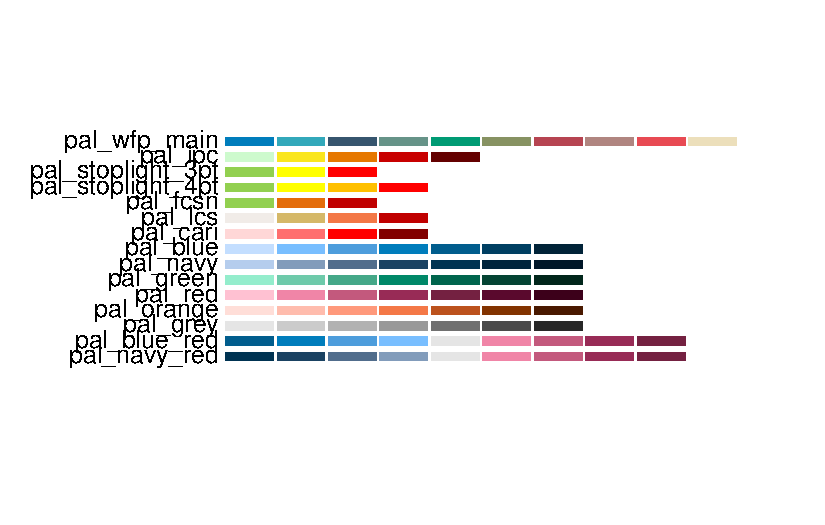
\includegraphics{chapter_five_files/figure-pdf/unnamed-chunk-2-1.pdf}

}

\end{figure}

\hypertarget{visualizing-outcome-indicators}{%
\section{Visualizing Outcome
Indicators}\label{visualizing-outcome-indicators}}

\hypertarget{food-consumption-score}{%
\subsection{Food Consumption Score}\label{food-consumption-score}}

\begin{Shaded}
\begin{Highlighting}[]
\FunctionTok{val\_lab}\NormalTok{(indicators\_data}\SpecialCharTok{$}\NormalTok{FCSCat) }\OtherTok{=} \FunctionTok{num\_lab}\NormalTok{(}\StringTok{"}
\StringTok{             1 Poor}
\StringTok{             2 Borderline}
\StringTok{             3 Acceptable}
\StringTok{"}\NormalTok{)}

\NormalTok{fcscat21\_admin1\_table\_long }\OtherTok{\textless{}{-}}\NormalTok{ indicators\_data }\SpecialCharTok{\%\textgreater{}\%} 
  \FunctionTok{group\_by}\NormalTok{(}\AttributeTok{ADMIN1Name\_lab =} \FunctionTok{to\_factor}\NormalTok{(ADMIN1Name)) }\SpecialCharTok{\%\textgreater{}\%}
  \FunctionTok{count}\NormalTok{(}\AttributeTok{FCSCat21\_lab =} \FunctionTok{as.character}\NormalTok{(FCSCat)) }\SpecialCharTok{\%\textgreater{}\%}
  \FunctionTok{mutate}\NormalTok{(}\AttributeTok{perc =} \DecValTok{100} \SpecialCharTok{*}\NormalTok{ n }\SpecialCharTok{/} \FunctionTok{sum}\NormalTok{(n)) }\SpecialCharTok{\%\textgreater{}\%}
  \FunctionTok{ungroup}\NormalTok{() }\SpecialCharTok{\%\textgreater{}\%} \FunctionTok{select}\NormalTok{(}\SpecialCharTok{{-}}\NormalTok{n) }\SpecialCharTok{\%\textgreater{}\%} \FunctionTok{mutate\_if}\NormalTok{(is.numeric, round, }\DecValTok{1}\NormalTok{) }
\end{Highlighting}
\end{Shaded}

\begin{Shaded}
\begin{Highlighting}[]
\CommentTok{\#create a palette of fcs based on wfpthemes palette and set ordering of values}
\NormalTok{pal\_fcs }\OtherTok{\textless{}{-}} \FunctionTok{wfp\_pal}\NormalTok{(}\StringTok{"pal\_stoplight\_3pt"}\NormalTok{, }\AttributeTok{n =} \DecValTok{3}\NormalTok{)}
\NormalTok{order\_fcs }\OtherTok{\textless{}{-}} \FunctionTok{c}\NormalTok{(}\StringTok{"Acceptable"}\NormalTok{, }\StringTok{"Borderline"}\NormalTok{, }\StringTok{"Poor"}\NormalTok{)}
\NormalTok{pal\_fcs }\OtherTok{\textless{}{-}} \FunctionTok{setNames}\NormalTok{(pal\_fcs, order\_fcs)}

\CommentTok{\#and now the graph {-} option1 {-} no y axis }
\NormalTok{fcscat21\_barplot }\OtherTok{\textless{}{-}}\NormalTok{ fcscat21\_admin1\_table\_long }\SpecialCharTok{\%\textgreater{}\%} 
  \FunctionTok{ggplot}\NormalTok{() }\SpecialCharTok{+}
  \FunctionTok{geom\_col}\NormalTok{(}
    \FunctionTok{aes}\NormalTok{(}\AttributeTok{x =} \FunctionTok{fct\_reorder2}\NormalTok{(ADMIN1Name\_lab,}
\NormalTok{                         perc,  }
\NormalTok{                         FCSCat21\_lab,}
\NormalTok{                         \textbackslash{}(x,y) }\FunctionTok{sum}\NormalTok{(x}\SpecialCharTok{*}\NormalTok{(y}\SpecialCharTok{==}\StringTok{"Acceptable"}\NormalTok{))), }
        \AttributeTok{y =}\NormalTok{ perc,}
        \AttributeTok{fill =} \FunctionTok{factor}\NormalTok{(FCSCat21\_lab,}\AttributeTok{level=}\NormalTok{order\_fcs)), }
    \AttributeTok{width =} \FloatTok{0.7}\NormalTok{) }\SpecialCharTok{+}
  \FunctionTok{geom\_text}\NormalTok{(}\FunctionTok{aes}\NormalTok{(}\AttributeTok{x =}\NormalTok{ ADMIN1Name\_lab,}
                \AttributeTok{y =}\NormalTok{ perc,}
                \AttributeTok{color =} \FunctionTok{factor}\NormalTok{(FCSCat21\_lab,}\AttributeTok{level=}\NormalTok{order\_fcs),}
                \AttributeTok{label =} \FunctionTok{paste0}\NormalTok{(perc, }\StringTok{"\%"}\NormalTok{)),}
            \AttributeTok{position =} \FunctionTok{position\_stack}\NormalTok{(}\AttributeTok{vjust =} \FloatTok{0.5}\NormalTok{),}
            \AttributeTok{show.legend =} \ConstantTok{FALSE}\NormalTok{,}
            \AttributeTok{size =} \DecValTok{10}\SpecialCharTok{/}\NormalTok{.pt) }\SpecialCharTok{+}
  \FunctionTok{scale\_color\_manual}\NormalTok{(}
    \AttributeTok{values =} \FunctionTok{c}\NormalTok{(main\_white, main\_black, main\_white)}
\NormalTok{  ) }\SpecialCharTok{+}
  \FunctionTok{labs}\NormalTok{(}\AttributeTok{tag =} \StringTok{"Figure 1"}\NormalTok{,}
       \AttributeTok{title =} \StringTok{"Household Food Consumption Score (FCS)"}\NormalTok{,}
       \AttributeTok{subtitle =} \StringTok{"Percentage of Households per FCS"}\NormalTok{,}
       \AttributeTok{caption =} \StringTok{"Source: RAM Survey 2025"}
\NormalTok{  ) }\SpecialCharTok{+}  \FunctionTok{scale\_fill\_manual}\NormalTok{(}\AttributeTok{values =}\NormalTok{ pal\_fcs) }\SpecialCharTok{+} \FunctionTok{theme\_wfp}\NormalTok{(}\AttributeTok{grid =} \ConstantTok{FALSE}\NormalTok{, }\AttributeTok{axis\_text =} \StringTok{"x"}\NormalTok{, }\AttributeTok{axis =}\NormalTok{ F, }\AttributeTok{axis\_title =}\NormalTok{ F) }\SpecialCharTok{+} \FunctionTok{theme}\NormalTok{(}\AttributeTok{text =} \FunctionTok{element\_text}\NormalTok{(}\AttributeTok{family =} \StringTok{"sans"}\NormalTok{))}


\CommentTok{\# }
\CommentTok{\# theme(text = element\_text(family = "sans"))}

\CommentTok{\# plot the graph }
\NormalTok{fcscat21\_barplot}
\end{Highlighting}
\end{Shaded}

\begin{figure}[H]

{\centering 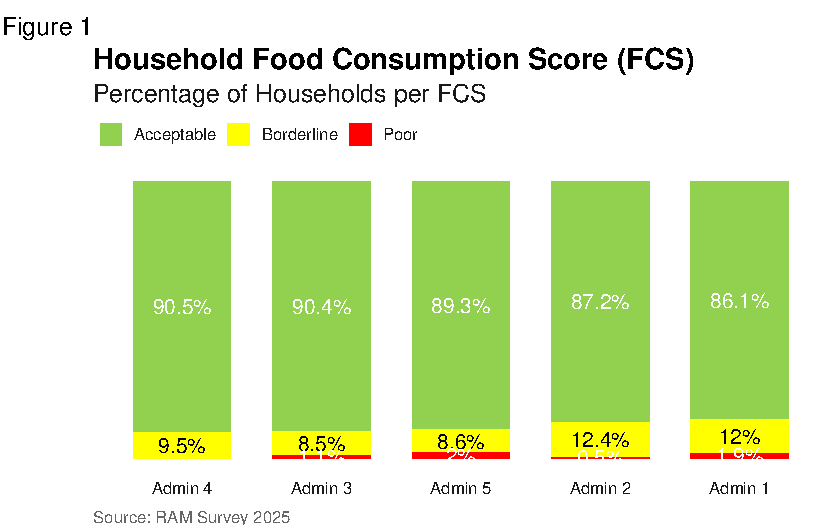
\includegraphics{chapter_five_files/figure-pdf/unnamed-chunk-4-1.pdf}

}

\end{figure}

\hypertarget{vitamin-a-rich-foods}{%
\subsection{Vitamin-A Rich Foods}\label{vitamin-a-rich-foods}}

\begin{Shaded}
\begin{Highlighting}[]
\NormalTok{indicators\_data}\SpecialCharTok{$}\NormalTok{ADMIN1Name }\OtherTok{\textless{}{-}}\NormalTok{ haven}\SpecialCharTok{::}\FunctionTok{as\_factor}\NormalTok{(indicators\_data}\SpecialCharTok{$}\NormalTok{ADMIN1Name)}

\CommentTok{\#set ordering}
\NormalTok{order\_fcsn }\OtherTok{\textless{}{-}} \FunctionTok{c}\NormalTok{(}\StringTok{"Consumed at least 7 times"}\NormalTok{,}\StringTok{"Consumed sometimes"}\NormalTok{,}\StringTok{"Never consumed"}\NormalTok{)}
\NormalTok{pal\_fcsn }\OtherTok{\textless{}{-}} \FunctionTok{setNames}\NormalTok{(pal\_fcsn, order\_fcsn )}

\CommentTok{\# create bar{-}chart for FGVitACat}
\NormalTok{percFGVitA\_admin1\_table\_long }\OtherTok{\textless{}{-}}\NormalTok{ indicators\_data }\SpecialCharTok{\%\textgreater{}\%}
  \FunctionTok{group\_by}\NormalTok{(}\AttributeTok{ADMIN1Name\_lab =} \FunctionTok{to\_factor}\NormalTok{(ADMIN1Name), }\AttributeTok{FGVitACat\_lab =} \FunctionTok{as.character}\NormalTok{(FGVitACat)) }\SpecialCharTok{\%\textgreater{}\%} 
  \FunctionTok{summarize}\NormalTok{(}\AttributeTok{count =} \FunctionTok{n}\NormalTok{()) }\SpecialCharTok{\%\textgreater{}\%}
  \FunctionTok{group\_by}\NormalTok{(ADMIN1Name\_lab) }\SpecialCharTok{\%\textgreater{}\%}
  \FunctionTok{mutate}\NormalTok{(}\AttributeTok{perc =} \FunctionTok{round}\NormalTok{(count}\SpecialCharTok{/}\FunctionTok{sum}\NormalTok{(count) }\SpecialCharTok{*} \DecValTok{100}\NormalTok{, }\DecValTok{1}\NormalTok{))}
\end{Highlighting}
\end{Shaded}

\begin{verbatim}
`summarise()` has grouped output by 'ADMIN1Name_lab'. You can override using
the `.groups` argument.
\end{verbatim}

\begin{Shaded}
\begin{Highlighting}[]
\NormalTok{percFGVitA\_barplot }\OtherTok{\textless{}{-}}\NormalTok{ percFGVitA\_admin1\_table\_long }\SpecialCharTok{\%\textgreater{}\%} 
  \FunctionTok{ggplot}\NormalTok{() }\SpecialCharTok{+}
  \FunctionTok{geom\_col}\NormalTok{(}
    \FunctionTok{aes}\NormalTok{(}\AttributeTok{x =} \FunctionTok{fct\_reorder2}\NormalTok{(ADMIN1Name\_lab,}
\NormalTok{                         perc,  }
\NormalTok{                         FGVitACat\_lab,}
\NormalTok{                         \textbackslash{}(x,y) }\FunctionTok{sum}\NormalTok{(x}\SpecialCharTok{*}\NormalTok{(y}\SpecialCharTok{==}\StringTok{"Consumed at least 7 times"}\NormalTok{))), }
        \AttributeTok{y =}\NormalTok{ perc,}
        \AttributeTok{fill =} \FunctionTok{factor}\NormalTok{(FGVitACat\_lab, }\AttributeTok{level=}\NormalTok{order\_fcsn)), }
    \AttributeTok{width =} \FloatTok{0.7}\NormalTok{) }\SpecialCharTok{+}
  \FunctionTok{geom\_text}\NormalTok{(}\FunctionTok{aes}\NormalTok{(}\AttributeTok{x =}\NormalTok{ ADMIN1Name\_lab,}
                \AttributeTok{y =}\NormalTok{ perc,}
                \AttributeTok{color =} \FunctionTok{factor}\NormalTok{(FGVitACat\_lab, }\AttributeTok{level=}\NormalTok{order\_fcsn),}
                \AttributeTok{label =} \FunctionTok{paste0}\NormalTok{(perc, }\StringTok{"\%"}\NormalTok{)),}
            \AttributeTok{position =} \FunctionTok{position\_stack}\NormalTok{(}\AttributeTok{vjust =} \FloatTok{0.5}\NormalTok{),}
            \AttributeTok{show.legend =} \ConstantTok{FALSE}\NormalTok{,}
            \AttributeTok{size =} \DecValTok{10}\SpecialCharTok{/}\NormalTok{.pt) }\SpecialCharTok{+}
  \FunctionTok{scale\_color\_manual}\NormalTok{(}
    \AttributeTok{values =} \FunctionTok{c}\NormalTok{(main\_white, main\_black, main\_white)}
\NormalTok{  ) }\SpecialCharTok{+}
  \FunctionTok{labs}\NormalTok{(}\AttributeTok{tag =} \StringTok{"Figure"}\NormalTok{,}
       \AttributeTok{title =} \StringTok{"Household Food Consumption Nutritional Analysis by Target Group"}\NormalTok{,}
       \AttributeTok{subtitle =} \StringTok{"Percentage of Households Consuming Vitamin{-}A Rich Foods"}\NormalTok{,}
       \AttributeTok{caption =} \StringTok{"Source: PMLE Outcome Monitoring, data collected May 2023"}
\NormalTok{  ) }\SpecialCharTok{+}  \FunctionTok{scale\_fill\_manual}\NormalTok{(}\AttributeTok{values =}\NormalTok{ pal\_fcsn) }\SpecialCharTok{+} \FunctionTok{theme\_wfp}\NormalTok{(}\AttributeTok{grid =} \ConstantTok{FALSE}\NormalTok{, }\AttributeTok{axis\_text =} \StringTok{"x"}\NormalTok{, }\AttributeTok{axis =}\NormalTok{ F, }\AttributeTok{axis\_title =}\NormalTok{ F) }\SpecialCharTok{+} \FunctionTok{theme}\NormalTok{(}\AttributeTok{text =} \FunctionTok{element\_text}\NormalTok{(}\AttributeTok{family =} \StringTok{"sans"}\NormalTok{))}

\NormalTok{percFGVitA\_barplot}
\end{Highlighting}
\end{Shaded}

\begin{figure}[H]

{\centering 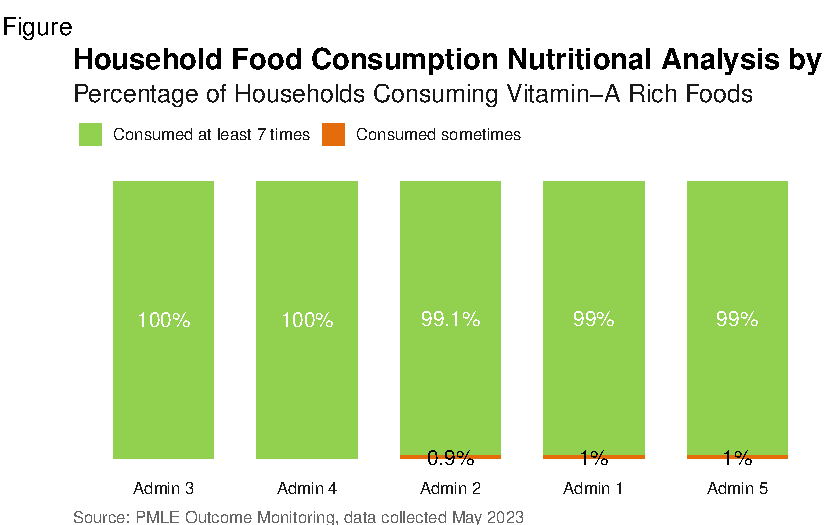
\includegraphics{chapter_five_files/figure-pdf/unnamed-chunk-5-1.pdf}

}

\end{figure}

\hypertarget{reduced-coping-strategies}{%
\subsection{Reduced Coping Strategies}\label{reduced-coping-strategies}}

\begin{Shaded}
\begin{Highlighting}[]
\NormalTok{data }\OtherTok{\textless{}{-}}\NormalTok{ sampledataenglish }\SpecialCharTok{\%\textgreater{}\%} \FunctionTok{mutate}\NormalTok{(}\AttributeTok{rCSI =}\NormalTok{ rCSILessQlty }\SpecialCharTok{+} 
\NormalTok{                          (rCSIBorrow }\SpecialCharTok{*} \DecValTok{2}\NormalTok{) }\SpecialCharTok{+} 
\NormalTok{                          rCSIMealNb }\SpecialCharTok{+} 
\NormalTok{                          rCSIMealSize }\SpecialCharTok{+} 
\NormalTok{                          (rCSIMealAdult }\SpecialCharTok{*} \DecValTok{3}\NormalTok{))}

\CommentTok{\# Create table of rCSI by ADMIN1 (unweighted) {-}{-}{-}{-}{-}{-}{-}{-}{-}{-}{-}{-}{-}{-}{-}{-}{-}{-}{-}{-}{-}{-}{-}{-}{-}{-}{-}{-}{-}{-}{-}{-}{-}{-}{-}{-}{-}{-}{-}{-}{-}{-}{-}{-}{-}{-}\#}

\NormalTok{rcsi\_admin1\_table\_long }\OtherTok{\textless{}{-}}\NormalTok{ data }\SpecialCharTok{\%\textgreater{}\%} 
  \FunctionTok{mutate}\NormalTok{(}\AttributeTok{ADMIN1Name\_lab =} \FunctionTok{to\_factor}\NormalTok{(ADMIN1Name)) }\SpecialCharTok{\%\textgreater{}\%} 
  \FunctionTok{group\_by}\NormalTok{(ADMIN1Name\_lab) }\SpecialCharTok{\%\textgreater{}\%} 
  \FunctionTok{drop\_na}\NormalTok{(rCSI) }\SpecialCharTok{\%\textgreater{}\%}   
  \FunctionTok{summarise}\NormalTok{(}\AttributeTok{meanrCSI =} \FunctionTok{round}\NormalTok{(}\FunctionTok{mean}\NormalTok{(rCSI),}\DecValTok{1}\NormalTok{))}
\end{Highlighting}
\end{Shaded}

\begin{Shaded}
\begin{Highlighting}[]
\NormalTok{rcsi\_barplot }\OtherTok{\textless{}{-}}\NormalTok{ rcsi\_admin1\_table\_long }\SpecialCharTok{\%\textgreater{}\%} \FunctionTok{ggplot}\NormalTok{() }\SpecialCharTok{+}
  \FunctionTok{geom\_col}\NormalTok{(}\FunctionTok{aes}\NormalTok{(}
    \AttributeTok{x =}\NormalTok{ meanrCSI,}
    \AttributeTok{y =} \FunctionTok{reorder}\NormalTok{(ADMIN1Name\_lab, meanrCSI),}
\NormalTok{  ),}
  \AttributeTok{fill =} \FunctionTok{wfp\_pal}\NormalTok{(}\AttributeTok{n =} \DecValTok{1}\NormalTok{, }\StringTok{"pal\_blue"}\NormalTok{),}
  \AttributeTok{width =} \FloatTok{0.8}
\NormalTok{  ) }\SpecialCharTok{+}
  \FunctionTok{labs}\NormalTok{(}
    \AttributeTok{tag =} \StringTok{"Figure 7"}\NormalTok{,}
    \AttributeTok{title =} \StringTok{"Reduced Coping Strategy Index (rCSI) by State | April 2023"}\NormalTok{,}
    \AttributeTok{subtitle =} \StringTok{"Average rCSI  per Household by State"}\NormalTok{,}
    \AttributeTok{x =} \StringTok{"rCSI"}\NormalTok{,}
    \AttributeTok{y =} \StringTok{"State"}\NormalTok{,}
    \AttributeTok{caption =} \StringTok{"Source: Emergency Food Security Assessment, data collected April 2023"}
\NormalTok{  ) }\SpecialCharTok{+} \FunctionTok{geom\_text}\NormalTok{(}\FunctionTok{aes}\NormalTok{(}\AttributeTok{x =}\NormalTok{ meanrCSI,}
                    \AttributeTok{y =}\NormalTok{ ADMIN1Name\_lab, }\AttributeTok{label =}\NormalTok{ meanrCSI),}
                \AttributeTok{hjust =} \SpecialCharTok{{-}}\FloatTok{0.5}\NormalTok{,}
                \AttributeTok{size =} \DecValTok{8} \SpecialCharTok{/}\NormalTok{ .pt}
\NormalTok{  ) }\SpecialCharTok{+}
  \FunctionTok{scale\_x\_continuous}\NormalTok{(}
    \AttributeTok{expand =} \FunctionTok{expansion}\NormalTok{(}\FunctionTok{c}\NormalTok{(}\DecValTok{0}\NormalTok{, }\FloatTok{0.1}\NormalTok{)),}
    \AttributeTok{breaks =} \FunctionTok{pretty\_breaks}\NormalTok{(}\AttributeTok{n =} \DecValTok{7}\NormalTok{),}
    \AttributeTok{labels =} \FunctionTok{label\_number}\NormalTok{()}
\NormalTok{  ) }\SpecialCharTok{+} \FunctionTok{theme\_wfp}\NormalTok{(}\AttributeTok{grid =} \ConstantTok{FALSE}\NormalTok{, }\AttributeTok{axis =} \StringTok{"y"}\NormalTok{, }\AttributeTok{axis\_title =} \ConstantTok{FALSE}\NormalTok{, }\AttributeTok{axis\_text =} \StringTok{"y"}\NormalTok{) }\SpecialCharTok{+} \FunctionTok{theme}\NormalTok{(}\AttributeTok{text =} \FunctionTok{element\_text}\NormalTok{(}\AttributeTok{family =} \StringTok{"sans"}\NormalTok{))}

\NormalTok{rcsi\_barplot}
\end{Highlighting}
\end{Shaded}

\begin{figure}[H]

{\centering 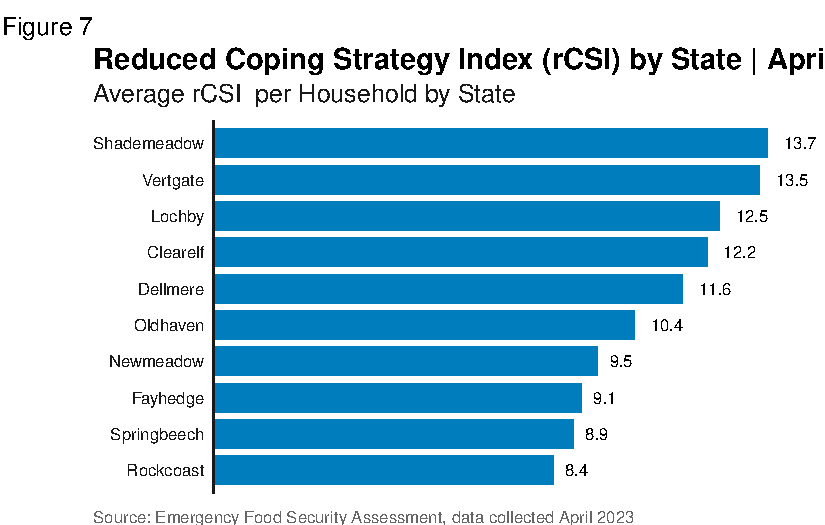
\includegraphics{chapter_five_files/figure-pdf/unnamed-chunk-7-1.pdf}

}

\end{figure}

\hypertarget{livelihood-coping-strategies}{%
\subsection{Livelihood Coping
Strategies}\label{livelihood-coping-strategies}}

\begin{Shaded}
\begin{Highlighting}[]
\NormalTok{indicators\_data }\OtherTok{\textless{}{-}}\NormalTok{ indicators\_data }\SpecialCharTok{\%\textgreater{}\%} 
  \FunctionTok{mutate}\NormalTok{(}\AttributeTok{LhCSI\_Category =} \FunctionTok{case\_when}\NormalTok{(}
\NormalTok{    Max\_coping\_behaviourFS }\SpecialCharTok{==} \StringTok{"Crisis coping strategies"} \SpecialCharTok{\textasciitilde{}} \StringTok{"Crisis"}\NormalTok{,}
\NormalTok{    Max\_coping\_behaviourFS }\SpecialCharTok{==} \StringTok{"Emergencies coping strategies"} \SpecialCharTok{\textasciitilde{}} \StringTok{"Emergency"}\NormalTok{,}
\NormalTok{    Max\_coping\_behaviourFS }\SpecialCharTok{==} \StringTok{"Stress coping strategies"} \SpecialCharTok{\textasciitilde{}} \StringTok{"Stress"}\NormalTok{,}
    \ConstantTok{TRUE} \SpecialCharTok{\textasciitilde{}} \StringTok{"Neutral"}
\NormalTok{  ))}


\CommentTok{\# Calculate the percentage of each level within each region area office}
\NormalTok{lcs\_admin1\_table\_long }\OtherTok{\textless{}{-}}\NormalTok{ indicators\_data }\SpecialCharTok{\%\textgreater{}\%} 
  \FunctionTok{group\_by}\NormalTok{(}\AttributeTok{ADMIN1Name\_lab =} \FunctionTok{to\_factor}\NormalTok{(ADMIN1Name)) }\SpecialCharTok{\%\textgreater{}\%}
  \FunctionTok{count}\NormalTok{(}\AttributeTok{Max\_coping\_behaviour\_FS\_lab =} \FunctionTok{as.character}\NormalTok{(LhCSI\_Category)) }\SpecialCharTok{\%\textgreater{}\%}
  \FunctionTok{mutate}\NormalTok{(}\AttributeTok{perc =} \DecValTok{100} \SpecialCharTok{*}\NormalTok{ n }\SpecialCharTok{/} \FunctionTok{sum}\NormalTok{(n)) }\SpecialCharTok{\%\textgreater{}\%}
  \FunctionTok{ungroup}\NormalTok{() }\SpecialCharTok{\%\textgreater{}\%} \FunctionTok{select}\NormalTok{(}\SpecialCharTok{{-}}\NormalTok{n) }\SpecialCharTok{\%\textgreater{}\%} \FunctionTok{mutate\_if}\NormalTok{(is.numeric, round, }\DecValTok{1}\NormalTok{) }

\CommentTok{\#this will make sure proper color gets assigned to proper value no mater how table of values was created}
\NormalTok{order\_lcs }\OtherTok{\textless{}{-}} \FunctionTok{c}\NormalTok{(}\StringTok{"Neutral"}\NormalTok{,}\StringTok{"Stress"}\NormalTok{,}\StringTok{"Crisis"}\NormalTok{,}\StringTok{"Emergency"}\NormalTok{)}
\NormalTok{pal\_lcs }\OtherTok{\textless{}{-}} \FunctionTok{setNames}\NormalTok{(pal\_lcs, order\_lcs)}

\CommentTok{\#and now the graph {-} option1 {-} no y axis }
\NormalTok{lcs\_barplot }\OtherTok{\textless{}{-}}\NormalTok{ lcs\_admin1\_table\_long }\SpecialCharTok{\%\textgreater{}\%} 
  \FunctionTok{ggplot}\NormalTok{() }\SpecialCharTok{+}
  \FunctionTok{geom\_col}\NormalTok{(}
    \FunctionTok{aes}\NormalTok{(}\AttributeTok{x =} \FunctionTok{fct\_reorder2}\NormalTok{(ADMIN1Name\_lab,}
\NormalTok{                         perc,  }
\NormalTok{                         Max\_coping\_behaviour\_FS\_lab,}
\NormalTok{                         \textbackslash{}(x,y) }\FunctionTok{sum}\NormalTok{(x}\SpecialCharTok{*}\NormalTok{(y}\SpecialCharTok{==}\StringTok{"Neutral"}\NormalTok{))), }
        \AttributeTok{y =}\NormalTok{ perc,}
        \AttributeTok{fill =} \FunctionTok{factor}\NormalTok{(Max\_coping\_behaviour\_FS\_lab,}\AttributeTok{level=}\NormalTok{order\_lcs)), }
    \AttributeTok{width =} \FloatTok{0.7}\NormalTok{) }\SpecialCharTok{+}
  \FunctionTok{geom\_text}\NormalTok{(}\FunctionTok{aes}\NormalTok{(}\AttributeTok{x =}\NormalTok{ ADMIN1Name\_lab,}
                \AttributeTok{y =}\NormalTok{ perc,}
                \AttributeTok{color =} \FunctionTok{factor}\NormalTok{(Max\_coping\_behaviour\_FS\_lab,}\AttributeTok{level=}\NormalTok{order\_lcs),}
                \AttributeTok{label =} \FunctionTok{paste0}\NormalTok{(perc, }\StringTok{"\%"}\NormalTok{)),}
            \AttributeTok{position =} \FunctionTok{position\_stack}\NormalTok{(}\AttributeTok{vjust =} \FloatTok{0.5}\NormalTok{),}
            \AttributeTok{show.legend =} \ConstantTok{FALSE}\NormalTok{,}
            \AttributeTok{size =} \DecValTok{10}\SpecialCharTok{/}\NormalTok{.pt) }\SpecialCharTok{+}
  \FunctionTok{scale\_color\_manual}\NormalTok{(}
    \AttributeTok{values =} \FunctionTok{c}\NormalTok{(main\_black, main\_black, main\_white, main\_white)}
\NormalTok{  ) }\SpecialCharTok{+}
  \FunctionTok{labs}\NormalTok{(}\AttributeTok{tag =} \StringTok{"Figure"}\NormalTok{,}
       \AttributeTok{title =} \StringTok{"Household Livelihood Coping Strategies (LCS) by Activity"}\NormalTok{,}
       \AttributeTok{subtitle =} \StringTok{"Percentage of Households per LCS groups per Activity"}\NormalTok{,}
       \AttributeTok{caption =} \StringTok{"Source: PMLE Outcome Monitoring, data collected May 2023"}
\NormalTok{  ) }\SpecialCharTok{+}  \FunctionTok{scale\_fill\_manual}\NormalTok{(}\AttributeTok{values =}\NormalTok{ pal\_lcs) }\SpecialCharTok{+} \FunctionTok{theme\_wfp}\NormalTok{(}\AttributeTok{grid =} \ConstantTok{FALSE}\NormalTok{, }\AttributeTok{axis\_text =} \StringTok{"x"}\NormalTok{, }\AttributeTok{axis =}\NormalTok{ F, }\AttributeTok{axis\_title =}\NormalTok{ F) }\SpecialCharTok{+}\FunctionTok{theme}\NormalTok{(}\AttributeTok{text =} \FunctionTok{element\_text}\NormalTok{(}\AttributeTok{family =} \StringTok{"sans"}\NormalTok{)) }

\NormalTok{lcs\_barplot}
\end{Highlighting}
\end{Shaded}

\begin{figure}[H]

{\centering 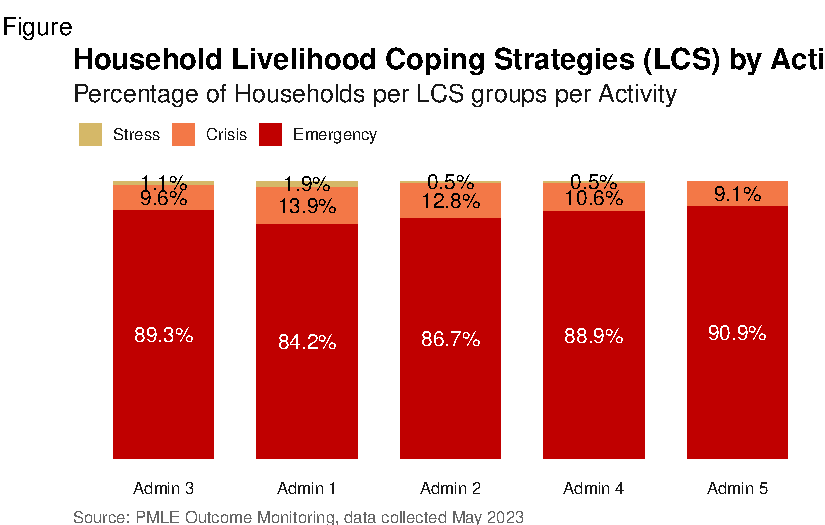
\includegraphics{chapter_five_files/figure-pdf/unnamed-chunk-8-1.pdf}

}

\end{figure}

\hypertarget{chart-types}{%
\section{Chart Types}\label{chart-types}}

\hypertarget{barcomumn-chart}{%
\subsection{Bar/Comumn Chart}\label{barcomumn-chart}}

\hypertarget{grouped-bar-chart}{%
\subsection{Grouped Bar Chart}\label{grouped-bar-chart}}

\begin{Shaded}
\begin{Highlighting}[]
\NormalTok{abi\_summary }\OtherTok{\textless{}{-}}\NormalTok{ indicators\_data }\SpecialCharTok{\%\textgreater{}\%} 
  \FunctionTok{group\_by}\NormalTok{(}\AttributeTok{ADMIN1Name\_lab =}\NormalTok{ labelled}\SpecialCharTok{::}\FunctionTok{to\_factor}\NormalTok{(HHHSex)) }\SpecialCharTok{\%\textgreater{}\%}
  \FunctionTok{count}\NormalTok{(}\AttributeTok{HHSNoFood\_lab =}\NormalTok{ labelled}\SpecialCharTok{::}\FunctionTok{to\_factor}\NormalTok{(ADMIN1Name)) }\SpecialCharTok{\%\textgreater{}\%}
  \FunctionTok{mutate}\NormalTok{(}\AttributeTok{perc =} \DecValTok{100} \SpecialCharTok{*}\NormalTok{ n }\SpecialCharTok{/} \FunctionTok{sum}\NormalTok{(n)) }\SpecialCharTok{\%\textgreater{}\%}
  \FunctionTok{ungroup}\NormalTok{() }\SpecialCharTok{\%\textgreater{}\%} \FunctionTok{select}\NormalTok{(}\SpecialCharTok{{-}}\NormalTok{n) }\SpecialCharTok{\%\textgreater{}\%} \FunctionTok{mutate\_if}\NormalTok{(is.numeric, round, }\DecValTok{1}\NormalTok{) }


\NormalTok{abi\_plot }\OtherTok{\textless{}{-}} \FunctionTok{ggplot}\NormalTok{(abi\_summary) }\SpecialCharTok{+}\FunctionTok{geom\_bar}\NormalTok{(}
  \FunctionTok{aes}\NormalTok{(}\AttributeTok{x =}\NormalTok{ ADMIN1Name\_lab, }\AttributeTok{y =}\NormalTok{ perc, }\AttributeTok{fill =}\NormalTok{ HHSNoFood\_lab, }\AttributeTok{group =}\NormalTok{ HHSNoFood\_lab), }
  \AttributeTok{stat=}\StringTok{\textquotesingle{}identity\textquotesingle{}}\NormalTok{, }\AttributeTok{position=}\FunctionTok{position\_dodge}\NormalTok{(.}\DecValTok{7}\NormalTok{),  }\AttributeTok{width =} \FloatTok{0.6}\NormalTok{,}
\NormalTok{) }\SpecialCharTok{+}
  \FunctionTok{geom\_text}\NormalTok{(}
    \FunctionTok{aes}\NormalTok{(}\AttributeTok{x =}\NormalTok{ ADMIN1Name\_lab, }\AttributeTok{y =}\NormalTok{ perc, }\AttributeTok{label =}\NormalTok{ perc, }\AttributeTok{group =}\NormalTok{ HHSNoFood\_lab),}
    \AttributeTok{position =} \FunctionTok{position\_dodge}\NormalTok{(}\AttributeTok{width =} \FloatTok{0.6}\NormalTok{),}
    \AttributeTok{vjust =} \SpecialCharTok{{-}}\FloatTok{0.5}\NormalTok{, }\AttributeTok{size =} \FloatTok{2.5}
\NormalTok{  )}\SpecialCharTok{+}
  \FunctionTok{scale\_fill\_wfp\_b}\NormalTok{(}\AttributeTok{palette =} \StringTok{"pal\_wfp\_main"}\NormalTok{) }\SpecialCharTok{+}
  \FunctionTok{labs}\NormalTok{(}
    \AttributeTok{title =} \StringTok{"Percentage of Households Reporting Benefit from Assets"}\NormalTok{,}
    \AttributeTok{subtitle =} \StringTok{""}\NormalTok{,}
    \AttributeTok{caption =} \StringTok{"Source: PMLE Outcome Monitoring, data collected May 2023"}
\NormalTok{  ) }\SpecialCharTok{+} \FunctionTok{theme\_wfp}\NormalTok{() }\SpecialCharTok{+}\FunctionTok{theme}\NormalTok{(}\AttributeTok{text =} \FunctionTok{element\_text}\NormalTok{(}\AttributeTok{family =} \StringTok{"sans"}\NormalTok{))}

\NormalTok{abi\_plot}
\end{Highlighting}
\end{Shaded}

\begin{figure}[H]

{\centering 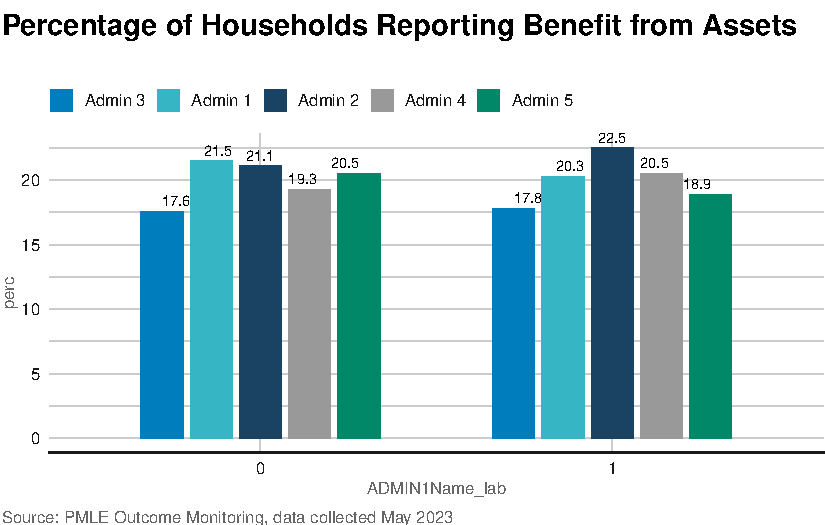
\includegraphics{chapter_five_files/figure-pdf/unnamed-chunk-9-1.pdf}

}

\end{figure}

\bookmarksetup{startatroot}

\hypertarget{reporting-dashboards}{%
\chapter{Reporting \& Dashboards}\label{reporting-dashboards}}

\hypertarget{reflections-session}{%
\section{Reflections Session}\label{reflections-session}}

You have now done the bigest part of the work and have analyzed data
with visualizations. therefdore you'll need to conduct reflection
session by inviting key stakeholders including programme teams and
partners to reflect on the preliminary results. at this stage, carefully
select the most relevent analysis and charts for interpreatation.in
order to keep participants focused, \textbf{a reflection session shall
not last more than 2 hours and include not more than 60 slides}

\hypertarget{take-reflections-note}{%
\subsection{Take Reflections Note}\label{take-reflections-note}}

\begin{itemize}
\tightlist
\item
  Reflect: question data quality and make suggestions to adjust and
  identify additional cleaning steps
\item
  Interpret: develop qualitative intepretations of data patterns
\item
  Recomend: suggest recomendations in terms of programming adjustments
\item
  Clasify: define level of sensitivity for certian topics if required
\end{itemize}

\hypertarget{using-data-library}{%
\section{Using Data Library}\label{using-data-library}}

\texttt{Data\ Library} is WFP's secure space for indexing, versioning
and storing data. this service is easy to use and is backed by WFP
enterpreice security, management tools, policies and procedures. using
the Data Library servies three purposes:

\begin{itemize}
\tightlist
\item
  it helps standrize formating of country office (CO) household survey
  datasets and metadata
\item
  it functions as a secure, presistenty storage for all CO household
  survey data and as a repository of survey reports
\item
  while the data ownership statys with the country office, Data Library
  enables sharing of specefic relevent datasets and reports with wider
  audinces such as Regional Bureaus and Headquarters for global analysis
  and even with parnters and donors for knowledge sharing and
  accountability.
\end{itemize}

\hypertarget{how-to-package-your-project}{%
\subsection{How to Package your
Project}\label{how-to-package-your-project}}

for each completed assessment and monitoring survey, CO should upload
the following informaton in Data Library, each in seperate folder. good
practice is to setup your working repository at the planning stage so
you can upload each file once completed.

\begin{enumerate}
\def\labelenumi{\arabic{enumi}.}
\tightlist
\item
  Raw Data
\item
  Sntax
\item
  Internal Processed Data
\item
  External Processed Data
\item
  Output Tables
\item
  Reports
\item
  TOR and Technical Notes
\item
  Questionnaire
\item
  Secondary Info
\item
  Miscellaneous
\end{enumerate}

\begin{quote}
The ambition of RAM is to make household food security and essential
needs assessment and monitoring survey data available as a public good
\end{quote}

\bookmarksetup{startatroot}

\hypertarget{references}{%
\chapter*{References}\label{references}}
\addcontentsline{toc}{chapter}{References}

\markboth{References}{References}

\hypertarget{refs}{}
\begin{CSLReferences}{0}{0}
\end{CSLReferences}



\end{document}
